\documentclass[11pt,a4paper]{article}
\setlength{\headheight}{14pt}
\usepackage[margin=1in]{geometry}
\usepackage{amsmath}
\usepackage{amssymb}
\usepackage{titlesec}
\usepackage{enumitem}
\usepackage{xcolor}
\usepackage[most]{tcolorbox}
\usepackage{fancyhdr}
\usepackage{listings}
\usepackage{hyperref}
\usepackage{graphicx}
\usepackage{tikz}
\usetikzlibrary{shapes.geometric, arrows, positioning}

\newcommand{\wrongmark}{\times}
\usepackage[utf8]{inputenc}
\usepackage{newunicodechar} 
\newunicodechar{✓}{\checkmark}
\newunicodechar{✗}{\wrongmark}
\DeclareUnicodeCharacter{2502}{|}
\DeclareUnicodeCharacter{251C}{+}
\DeclareUnicodeCharacter{2500}{-}
\DeclareUnicodeCharacter{2514}{+}

% Header and Footer
\pagestyle{fancy}
\fancyhf{}
\rhead{MLOps Complete Guide}
\lhead{DVC, Git \& MLflow Integration}
\cfoot{\thepage}

% Title formatting
\titleformat{\section}{\Large\bfseries\color{blue!70!black}}{\thesection}{1em}{}[\titlerule]
\titleformat{\subsection}{\large\bfseries\color{blue!50!black}}{\thesubsection}{1em}{}
\titleformat{\subsubsection}{\normalsize\bfseries\color{blue!40!black}}{\thesubsubsection}{1em}{}

% Code styling
\definecolor{codebg}{gray}{0.95}
\definecolor{codegreen}{rgb}{0,0.6,0}
\definecolor{codegray}{rgb}{0.5,0.5,0.5}
\definecolor{codepurple}{rgb}{0.58,0,0.82}

\lstdefinestyle{pythonstyle}{
    language=Python,
    backgroundcolor=\color{codebg},
    commentstyle=\color{codegreen},
    keywordstyle=\color{blue},
    numberstyle=\tiny\color{codegray},
    stringstyle=\color{codepurple},
    basicstyle=\ttfamily\small,
    breaklines=true,
    captionpos=b,
    keepspaces=true,
    numbers=left,
    numbersep=5pt,
    showspaces=false,
    showstringspaces=false,
    showtabs=false,
    tabsize=4,
    frame=single,
    xleftmargin=2em,
    framexleftmargin=1.5em
}

\lstdefinestyle{bashstyle}{
    language=bash,
    backgroundcolor=\color{codebg},
    basicstyle=\ttfamily\small,
    breaklines=true,
    frame=single,
    xleftmargin=2em,
    framexleftmargin=1.5em
}

\lstdefinestyle{yamlstyle}{
    backgroundcolor=\color{codebg},
    basicstyle=\ttfamily\small,
    breaklines=true,
    frame=single,
    xleftmargin=2em,
    framexleftmargin=1.5em
}

\lstset{style=pythonstyle}

% Command box
\newtcolorbox{cmdbox}{
    colback=codebg,
    colframe=black!50,
    boxrule=0.5pt,
    left=2mm,
    right=2mm,
    top=1mm,
    bottom=1mm,
    breakable,
    enhanced jigsaw
}

% Example box
\newtcolorbox{examplebox}[1]{
    colback=green!5!white,
    colframe=green!75!black,
    title=#1,
    fonttitle=\bfseries,
    breakable,
    enhanced jigsaw
}

% Note box
\newtcolorbox{notebox}{
    colback=yellow!10!white,
    colframe=orange!75!black,
    title=Important Note,
    fonttitle=\bfseries,
    breakable,
    enhanced jigsaw
}

% Warning box
\newtcolorbox{warningbox}{
    colback=red!5!white,
    colframe=red!75!black,
    title=Warning,
    fonttitle=\bfseries,
    breakable,
    enhanced jigsaw
}

% Info box
\newtcolorbox{infobox}[1]{
    colback=blue!5!white,
    colframe=blue!75!black,
    title=#1,
    fonttitle=\bfseries,
    breakable,
    enhanced jigsaw
}

\begin{document}

% Title Page
\begin{titlepage}
    \centering
    \vspace*{2cm}
    {\Huge\bfseries MLOps Project\\[0.5cm] with DVC, Git \& MLflow\par}
    \vspace{1cm}
    {\Large Complete Integration Guide\par}
    \vspace{2cm}
    {\large A Comprehensive Guide to Building Production MLOps\\
    Pipelines with DVC Version Control, Git Integration,\\
    and MLflow Experiment Tracking via DagShub\par}
    \vspace{3cm}
    {\Large\bfseries Sujil S\par}
    \vspace{0.5cm}
    {\large\texttt{sujil9480@gmail.com}\par}
    \vfill
    {\large \today\par}
\end{titlepage}

\tableofcontents
\newpage

% ========================
% SECTION 1: INTRODUCTION
% ========================
\section{Introduction to MLOps with DagShub}

\subsection{What is This Project About?}

This comprehensive guide demonstrates a complete MLOps workflow that integrates three powerful tools:

\begin{enumerate}[leftmargin=*]
    \item \textbf{DVC (Data Version Control)}: For versioning data, models, and pipeline artifacts
    \item \textbf{Git}: For versioning code and metadata
    \item \textbf{MLflow via DagShub}: For experiment tracking and model registry
\end{enumerate}

\begin{infobox}{Project Goals}
By the end of this guide, you will:
\begin{itemize}[leftmargin=*]
    \item Build a complete ML pipeline with proper logging
    \item Version control data and models with DVC
    \item Track experiments with MLflow on DagShub
    \item Compare multiple model runs systematically
    \item Freeze and deploy the best performing model
    \item Enable team collaboration and reproducibility
\end{itemize}
\end{infobox}

\subsection{The MLOps Stack}

\begin{center}
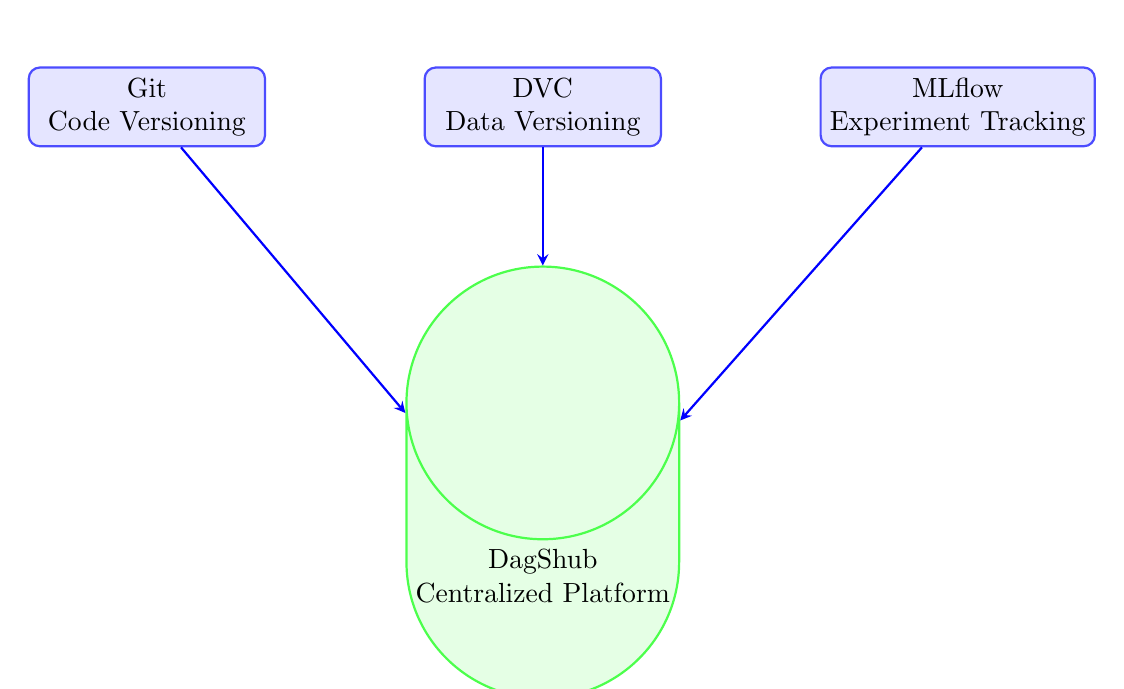
\begin{tikzpicture}[
    node distance=2cm,
    box/.style={rectangle, rounded corners, draw=blue!70, fill=blue!10, thick, minimum width=3cm, minimum height=1cm, align=center},
    storage/.style={cylinder, shape border rotate=90, draw=green!70, fill=green!10, thick, minimum width=2.5cm, minimum height=1.2cm, align=center},
    arrow/.style={->, >=stealth, thick, blue}
]

\node[box] (git) {Git\\Code Versioning};
\node[box, right=of git] (dvc) {DVC\\Data Versioning};
\node[box, right=of dvc] (mlflow) {MLflow\\Experiment Tracking};
\node[storage, below=1.5cm of dvc] (dagshub) {DagShub\\Centralized Platform};

\draw[arrow] (git) -- (dagshub);
\draw[arrow] (dvc) -- (dagshub);
\draw[arrow] (mlflow) -- (dagshub);

\end{tikzpicture}
\end{center}

\subsection{What Makes This Different?}

Unlike the previous DVC-only workflow, this project adds:

\begin{itemize}[leftmargin=*]
    \item \textbf{Centralized Experiment Tracking}: MLflow UI hosted on DagShub
    \item \textbf{Team Collaboration}: Everyone sees all experiments
    \item \textbf{Model Comparison}: Visual comparison of multiple runs
    \item \textbf{Experiment Tagging}: Link Git commits to MLflow runs
    \item \textbf{Model Registry}: Track model lineage and deployment status
\end{itemize}

\subsection{Key Differences from Previous Workflow}

\begin{center}
\begin{tabular}{|p{0.45\textwidth}|p{0.45\textwidth}|}
\hline
\textbf{DVC-Only Workflow} & \textbf{DVC + MLflow Workflow} \\
\hline
Local experiment tracking & Centralized MLflow tracking \\
\hline
Manual metric comparison & Visual metric comparison \\
\hline
Experiments private to user & All experiments visible to team \\
\hline
Limited experiment history & Full experiment history preserved \\
\hline
No model registry & MLflow model registry \\
\hline
\end{tabular}
\end{center}

\newpage

% ========================
% SECTION 2: SETUP
% ========================
\section{Initial Project Setup}

\subsection{Step 1: Create Python Environment}

\begin{cmdbox}
\begin{verbatim}
# Create virtual environment
python -m venv venv
\end{verbatim}
\end{cmdbox}

\subsection{Step 2: Activate Environment}

\begin{cmdbox}
\begin{verbatim}
# Windows
venv\Scripts\activate.bat

# Linux/Mac
source venv/bin/activate
\end{verbatim}
\end{cmdbox}

\subsection{Step 3: Create Source Directory}

\begin{cmdbox}
\begin{verbatim}
mkdir src
\end{verbatim}
\end{cmdbox}

\subsection{Step 4: Create Requirements File}

\begin{examplebox}{requirements.txt}
\begin{verbatim}
dvc
numpy
pandas
matplotlib
wordcloud
nltk
scikit-learn
xgboost
pyyaml
mlflow
dagshub
\end{verbatim}
\end{examplebox}

\begin{notebox}
\textbf{New Dependencies}:
\begin{itemize}[leftmargin=*]
    \item \textbf{mlflow}: Experiment tracking library
    \item \textbf{dagshub}: DagShub integration for MLflow
    \item \textbf{xgboost}: Additional model option (if needed)
\end{itemize}
\end{notebox}

\subsection{Step 5: Install Requirements}

\begin{cmdbox}
\begin{verbatim}
pip install -r requirements.txt
\end{verbatim}
\end{cmdbox}

\newpage

% ========================
% SECTION 3: PIPELINE COMPONENTS
% ========================
\section{Building Pipeline Components}

\subsection{Component Overview}

The ML pipeline consists of five stages:

\begin{enumerate}[leftmargin=*]
    \item \textbf{Data Ingestion}: Load and split data
    \item \textbf{Data Pre-Processing}: Clean and transform text
    \item \textbf{Feature Engineering}: Apply TF-IDF
    \item \textbf{Model Building}: Train RandomForest
    \item \textbf{Model Evaluation}: Calculate metrics and log to MLflow
\end{enumerate}

\subsection{Data Ingestion Module}

\begin{examplebox}{src/Data\_Ingestion.py}
\begin{lstlisting}[language=Python]
import pandas as pd
import os
from sklearn.model_selection import train_test_split
import logging
import yaml

# Ensure the "logs" directory exists
log_dir = 'logs'
os.makedirs(log_dir, exist_ok=True)

# Logging configuration
logger = logging.getLogger('Data_Ingestion')
logger.setLevel('DEBUG')

console_handler = logging.StreamHandler()
console_handler.setLevel('DEBUG')

log_file_path = os.path.join(log_dir, 'Data_Ingestion.log')
file_handler = logging.FileHandler(log_file_path)
file_handler.setLevel('DEBUG')

formatter = logging.Formatter(
    '%(asctime)s - %(name)s - %(levelname)s - %(message)s'
)
console_handler.setFormatter(formatter)
file_handler.setFormatter(formatter)

logger.addHandler(console_handler)
logger.addHandler(file_handler)


def load_params(params_path: str) -> dict:
    """Load parameters from a YAML file."""
    try:
        with open(params_path, 'r') as file:
            params = yaml.safe_load(file)
        logger.debug('Parameters retrieved from %s', params_path)
        return params
    except FileNotFoundError:
        logger.error('File not found: %s', params_path)
        raise
    except yaml.YAMLError as e:
        logger.error('YAML error: %s', e)
        raise
    except Exception as e:
        logger.error('Unexpected error: %s', e)
        raise


def load_data(data_url: str) -> pd.DataFrame:
    """Load data from a CSV file."""
    try:
        df = pd.read_csv(data_url)
        logger.debug('Data loaded from %s', data_url)
        return df
    except pd.errors.ParserError as e:
        logger.error('Failed to parse the CSV file: %s', e)
        raise
    except Exception as e:
        logger.error('Unexpected error while loading data: %s', e)
        raise


def preprocess_data(df: pd.DataFrame) -> pd.DataFrame:
    """Preprocess the data."""
    try:
        df.drop(columns=['Unnamed: 2', 'Unnamed: 3', 'Unnamed: 4'], 
                inplace=True)
        df.rename(columns={'v1': 'target', 'v2': 'text'}, 
                  inplace=True)
        logger.debug('Data preprocessing completed')
        return df
    except KeyError as e:
        logger.error('Missing column in dataframe: %s', e)
        raise
    except Exception as e:
        logger.error('Unexpected error during preprocessing: %s', e)
        raise


def save_data(train_data: pd.DataFrame, 
              test_data: pd.DataFrame, 
              data_path: str) -> None:
    """Save the train and test datasets."""
    try:
        raw_data_path = os.path.join(data_path, 'raw')
        os.makedirs(raw_data_path, exist_ok=True)
        
        train_data.to_csv(
            os.path.join(raw_data_path, "train.csv"), 
            index=False
        )
        test_data.to_csv(
            os.path.join(raw_data_path, "test.csv"), 
            index=False
        )
        logger.debug('Train and test data saved to %s', 
                     raw_data_path)
    except Exception as e:
        logger.error('Error while saving data: %s', e)
        raise


def main():
    try:
        params = load_params(params_path='params.yaml')
        test_size = params['data_ingestion']['test_size']
        
        data_path = 'https://raw.githubusercontent.com/' \
                    'Error-Makes-Clever/MLOPS-Data-Versioning-' \
                    'using-DVC-Project-1/refs/heads/main/' \
                    'Experiments/spam.csv'
        
        df = load_data(data_url=data_path)
        final_df = preprocess_data(df)
        
        train_data, test_data = train_test_split(
            final_df, test_size=test_size, random_state=2
        )
        
        save_data(train_data, test_data, data_path='./data')
    except Exception as e:
        logger.error('Failed to complete data ingestion: %s', e)
        print(f"Error: {e}")


if __name__ == '__main__':
    main()
\end{lstlisting}
\end{examplebox}

\subsection{Data Pre-Processing Module}

\begin{examplebox}{src/Data\_Pre\_Processing.py - Part 1}
\begin{lstlisting}[language=Python]
import os
import logging
import pandas as pd
from sklearn.preprocessing import LabelEncoder
from nltk.stem.porter import PorterStemmer
from nltk.corpus import stopwords
import string
import nltk

nltk.download('stopwords')
nltk.download('punkt')

# Ensure the "logs" directory exists
log_dir = 'logs'
os.makedirs(log_dir, exist_ok=True)

# Setting up logger
logger = logging.getLogger('Data_Pre_Processing')
logger.setLevel('DEBUG')

console_handler = logging.StreamHandler()
console_handler.setLevel('DEBUG')

log_file_path = os.path.join(log_dir, 'Data_Pre_Processing.log')
file_handler = logging.FileHandler(log_file_path)
file_handler.setLevel('DEBUG')

formatter = logging.Formatter(
    '%(asctime)s - %(name)s - %(levelname)s - %(message)s'
)
console_handler.setFormatter(formatter)
file_handler.setFormatter(formatter)

logger.addHandler(console_handler)
logger.addHandler(file_handler)


def transform_text(text):
    """
    Transform text: lowercase, tokenize, remove stopwords,
    punctuation, and stem.
    """
    ps = PorterStemmer()
    
    # Convert to lowercase
    text = text.lower()
    
    # Tokenize
    text = nltk.word_tokenize(text)
    
    # Remove non-alphanumeric tokens
    text = [word for word in text if word.isalnum()]
    
    # Remove stopwords and punctuation
    text = [word for word in text 
            if word not in stopwords.words('english') 
            and word not in string.punctuation]
    
    # Stem the words
    text = [ps.stem(word) for word in text]
    
    # Join back into string
    return " ".join(text)


def preprocess_df(df, text_column='text', 
                  target_column='target'):
    """
    Preprocess DataFrame: encode target, remove duplicates,
    transform text.
    """
    try:
        logger.debug('Starting preprocessing for DataFrame')
        
        # Encode the target column
        encoder = LabelEncoder()
        df[target_column] = encoder.fit_transform(df[target_column])
        logger.debug('Target column encoded')
        
        # Remove duplicate rows
        df = df.drop_duplicates(keep='first')
        logger.debug('Duplicates removed')
        
        # Apply text transformation
        df.loc[:, text_column] = df[text_column].apply(
            transform_text
        )
        logger.debug('Text column transformed')
        
        return df
    except KeyError as e:
        logger.error('Column not found: %s', e)
        raise
    except Exception as e:
        logger.error('Error during text normalization: %s', e)
        raise


def main(text_column='text', target_column='target'):
    """
    Main function: load raw data, preprocess, save processed.
    """
    try:
        # Load data from data/raw
        train_data = pd.read_csv('./data/raw/train.csv')
        test_data = pd.read_csv('./data/raw/test.csv')
        logger.debug('Data loaded properly')
        
        # Transform the data
        train_processed = preprocess_df(train_data, 
                                        text_column, 
                                        target_column)
        test_processed = preprocess_df(test_data, 
                                       text_column, 
                                       target_column)
        
        # Store in data/interim
        data_path = os.path.join("./data", "interim")
        os.makedirs(data_path, exist_ok=True)
        
        train_processed.to_csv(
            os.path.join(data_path, "train_processed.csv"), 
            index=False
        )
        test_processed.to_csv(
            os.path.join(data_path, "test_processed.csv"),
            index=False
        )
        
        logger.debug('Processed data saved to %s', data_path)
    except FileNotFoundError as e:
        logger.error('File not found: %s', e)
    except pd.errors.EmptyDataError as e:
        logger.error('No data: %s', e)
    except Exception as e:
        logger.error('Failed to complete data transformation: %s', e)
        print(f"Error: {e}")


if __name__ == '__main__':
    main()
\end{lstlisting}
\end{examplebox}

\subsection{Feature Engineering Module}

\begin{examplebox}{src/Feature\_Engineering.py}
\begin{lstlisting}[language=Python]
import pandas as pd
import os
from sklearn.feature_extraction.text import TfidfVectorizer
import logging
import yaml

# Ensure the "logs" directory exists
log_dir = 'logs'
os.makedirs(log_dir, exist_ok=True)

# Logging configuration
logger = logging.getLogger('Feature_Engineering')
logger.setLevel('DEBUG')

console_handler = logging.StreamHandler()
console_handler.setLevel('DEBUG')

log_file_path = os.path.join(log_dir, 'Feature_Engineering.log')
file_handler = logging.FileHandler(log_file_path)
file_handler.setLevel('DEBUG')

formatter = logging.Formatter(
    '%(asctime)s - %(name)s - %(levelname)s - %(message)s'
)
console_handler.setFormatter(formatter)
file_handler.setFormatter(formatter)

logger.addHandler(console_handler)
logger.addHandler(file_handler)


def load_params(params_path: str) -> dict:
    """Load parameters from a YAML file."""
    try:
        with open(params_path, 'r') as file:
            params = yaml.safe_load(file)
        logger.debug('Parameters retrieved from %s', params_path)
        return params
    except FileNotFoundError:
        logger.error('File not found: %s', params_path)
        raise
    except yaml.YAMLError as e:
        logger.error('YAML error: %s', e)
        raise
    except Exception as e:
        logger.error('Unexpected error: %s', e)
        raise


def load_data(file_path: str) -> pd.DataFrame:
    """Load data from a CSV file."""
    try:
        df = pd.read_csv(file_path)
        df.fillna('', inplace=True)
        logger.debug('Data loaded and NaNs filled from %s', 
                     file_path)
        return df
    except pd.errors.ParserError as e:
        logger.error('Failed to parse the CSV file: %s', e)
        raise
    except Exception as e:
        logger.error('Unexpected error while loading data: %s', e)
        raise


def apply_tfidf(train_data: pd.DataFrame, 
                test_data: pd.DataFrame, 
                max_features: int) -> tuple:
    """Apply TF-IDF to the data."""
    try:
        vectorizer = TfidfVectorizer(max_features=max_features)
        
        X_train = train_data['text'].values
        y_train = train_data['target'].values
        X_test = test_data['text'].values
        y_test = test_data['target'].values
        
        X_train_bow = vectorizer.fit_transform(X_train)
        X_test_bow = vectorizer.transform(X_test)
        
        train_df = pd.DataFrame(X_train_bow.toarray())
        train_df['label'] = y_train
        
        test_df = pd.DataFrame(X_test_bow.toarray())
        test_df['label'] = y_test
        
        logger.debug('TF-IDF applied and data transformed')
        return train_df, test_df
    except Exception as e:
        logger.error('Error during TF-IDF transformation: %s', e)
        raise


def save_data(df: pd.DataFrame, file_path: str) -> None:
    """Save the dataframe to a CSV file."""
    try:
        os.makedirs(os.path.dirname(file_path), exist_ok=True)
        df.to_csv(file_path, index=False)
        logger.debug('Data saved to %s', file_path)
    except Exception as e:
        logger.error('Unexpected error while saving data: %s', e)
        raise


def main():
    try:
        params = load_params(params_path='params.yaml')
        max_features = params['feature_engineering']['max_features']
        
        train_data = load_data('./data/interim/train_processed.csv')
        test_data = load_data('./data/interim/test_processed.csv')
        
        train_df, test_df = apply_tfidf(train_data, test_data, 
                                        max_features)
        
        save_data(train_df, 
                  os.path.join("./data", "processed", 
                               "train_tfidf.csv"))
        save_data(test_df, 
                  os.path.join("./data", "processed", 
                               "test_tfidf.csv"))
    except Exception as e:
        logger.error('Failed to complete feature engineering: %s', e)
        print(f"Error: {e}")


if __name__ == '__main__':
    main()
\end{lstlisting}
\end{examplebox}

\subsection{Model Building Module}

\begin{examplebox}{src/Model\_Building\_Rf.py}
\begin{lstlisting}[language=Python]
import os
import numpy as np
import pandas as pd
import pickle
import logging
from sklearn.ensemble import RandomForestClassifier
import yaml

# Ensure the "logs" directory exists
log_dir = 'logs'
os.makedirs(log_dir, exist_ok=True)

# Logging configuration
logger = logging.getLogger('Model_Building')
logger.setLevel('DEBUG')

console_handler = logging.StreamHandler()
console_handler.setLevel('DEBUG')

log_file_path = os.path.join(log_dir, 'Model_Building.log')
file_handler = logging.FileHandler(log_file_path)
file_handler.setLevel('DEBUG')

formatter = logging.Formatter(
    '%(asctime)s - %(name)s - %(levelname)s - %(message)s'
)
console_handler.setFormatter(formatter)
file_handler.setFormatter(formatter)

logger.addHandler(console_handler)
logger.addHandler(file_handler)


def load_params(params_path: str) -> dict:
    """Load parameters from a YAML file."""
    try:
        with open(params_path, 'r') as file:
            params = yaml.safe_load(file)
        logger.debug('Parameters retrieved from %s', params_path)
        return params
    except FileNotFoundError:
        logger.error('File not found: %s', params_path)
        raise
    except yaml.YAMLError as e:
        logger.error('YAML error: %s', e)
        raise
    except Exception as e:
        logger.error('Unexpected error: %s', e)
        raise


def load_data(file_path: str) -> pd.DataFrame:
    """Load data from a CSV file."""
    try:
        df = pd.read_csv(file_path)
        logger.debug('Data loaded from %s with shape %s', 
                     file_path, df.shape)
        return df
    except pd.errors.ParserError as e:
        logger.error('Failed to parse the CSV file: %s', e)
        raise
    except FileNotFoundError as e:
        logger.error('File not found: %s', e)
        raise
    except Exception as e:
        logger.error('Unexpected error while loading data: %s', e)
        raise


def train_model(X_train: np.ndarray, 
                y_train: np.ndarray, 
                params: dict) -> RandomForestClassifier:
    """Train the RandomForest model."""
    try:
        if X_train.shape[0] != y_train.shape[0]:
            raise ValueError(
                "Number of samples in X_train and y_train must match"
            )
        
        logger.debug('Initializing RandomForest with params: %s', 
                     params)
        clf = RandomForestClassifier(
            n_estimators=params['n_estimators'],
            random_state=params['random_state'],
            max_depth=params['max_depth']
        )
        
        logger.debug('Model training started with %d samples', 
                     X_train.shape[0])
        clf.fit(X_train, y_train)
        logger.debug('Model training completed')
        
        return clf
    except ValueError as e:
        logger.error('ValueError during model training: %s', e)
        raise
    except Exception as e:
        logger.error('Error during model training: %s', e)
        raise


def save_model(model, file_path: str) -> None:
    """Save the trained model to a file."""
    try:
        os.makedirs(os.path.dirname(file_path), exist_ok=True)
        
        with open(file_path, 'wb') as file:
            pickle.dump(model, file)
        logger.debug('Model saved to %s', file_path)
    except FileNotFoundError as e:
        logger.error('File path not found: %s', e)
        raise
    except Exception as e:
        logger.error('Error while saving model: %s', e)
        raise


def main():
    try:
        params = load_params('params.yaml')['model_building']
        
        train_data = load_data('./data/processed/train_tfidf.csv')
        X_train = train_data.iloc[:, :-1].values
        y_train = train_data.iloc[:, -1].values
        
        clf = train_model(X_train, y_train, params)
        
        model_save_path = 'models/model_rf.pkl'
        save_model(clf, model_save_path)
        
    except Exception as e:
        logger.error('Failed to complete model building: %s', e)
        print(f"Error: {e}")


if __name__ == '__main__':
    main()
\end{lstlisting}
\end{examplebox}

\newpage

% ========================
% SECTION 4: MLFLOW INTEGRATION
% ========================
\section{MLflow Integration with DagShub}

\subsection{What is DagShub?}

\textbf{DagShub} is a platform for data scientists and ML engineers that provides:

\begin{itemize}[leftmargin=*]
    \item \textbf{Hosted MLflow}: No need to run your own MLflow server
    \item \textbf{Git Integration}: Direct connection to GitHub repositories
    \item \textbf{DVC Support}: Native DVC integration
    \item \textbf{Team Collaboration}: Shared experiment tracking
    \item \textbf{Free Tier}: Generous free plan for small teams
\end{itemize}

\subsection{Connecting to DagShub}

\subsubsection{Step 1: Create DagShub Account}

\begin{enumerate}[leftmargin=*]
    \item Go to \url{https://dagshub.com}
    \item Sign up with GitHub account
    \item Create a new repository or connect existing one
\end{enumerate}

\subsubsection{Step 2: Obtain Tracking URI}

After connecting your repository to DagShub:

\begin{cmdbox}
\begin{verbatim}
# Your tracking URI will look like:
https://dagshub.com/username/repo-name.mlflow
\end{verbatim}
\end{cmdbox}

\subsection{Model Evaluation with MLflow}

\begin{examplebox}{src/Model\_Evaluation\_Rf.py - Complete Implementation}
\begin{lstlisting}[language=Python]
import os
import numpy as np
import pandas as pd
import pickle
import json
from sklearn.metrics import (accuracy_score, precision_score, 
                             recall_score, roc_auc_score)
import logging
import mlflow
import yaml
import dagshub

# Initialize DagShub connection
dagshub.init(
    repo_owner='Error-Makes-Clever',
    repo_name='MLOPS-Dagshub-DVC-Git-Project',
    mlflow=True
)

# Set MLflow tracking URI
mlflow.set_tracking_uri(
    "https://dagshub.com/Error-Makes-Clever/"
    "MLOPS-Dagshub-DVC-Git-Project.mlflow"
)

# Set experiment name
mlflow.set_experiment("MLOPS-Project-with-Random-Forest")

# Ensure the "logs" directory exists
log_dir = 'logs'
os.makedirs(log_dir, exist_ok=True)

# Logging configuration
logger = logging.getLogger('Model_Evaluation')
logger.setLevel('DEBUG')

console_handler = logging.StreamHandler()
console_handler.setLevel('DEBUG')

log_file_path = os.path.join(log_dir, 'Model_Evaluation.log')
file_handler = logging.FileHandler(log_file_path)
file_handler.setLevel('DEBUG')

formatter = logging.Formatter(
    '%(asctime)s - %(name)s - %(levelname)s - %(message)s'
)
console_handler.setFormatter(formatter)
file_handler.setFormatter(formatter)

logger.addHandler(console_handler)
logger.addHandler(file_handler)


def load_params(params_path: str) -> dict:
    """Load parameters from a YAML file."""
    try:
        with open(params_path, 'r') as file:
            params = yaml.safe_load(file)
        logger.debug('Parameters retrieved from %s', params_path)
        return params
    except FileNotFoundError:
        logger.error('File not found: %s', params_path)
        raise
    except yaml.YAMLError as e:
        logger.error('YAML error: %s', e)
        raise
    except Exception as e:
        logger.error('Unexpected error: %s', e)
        raise


def load_model(file_path: str):
    """Load the trained model from a file."""
    try:
        with open(file_path, 'rb') as file:
            model = pickle.load(file)
        logger.debug('Model loaded from %s', file_path)
        return model
    except FileNotFoundError:
        logger.error('File not found: %s', file_path)
        raise
    except Exception as e:
        logger.error('Unexpected error while loading model: %s', e)
        raise


def load_data(file_path: str) -> pd.DataFrame:
    """Load data from a CSV file."""
    try:
        df = pd.read_csv(file_path)
        logger.debug('Data loaded from %s', file_path)
        return df
    except pd.errors.ParserError as e:
        logger.error('Failed to parse the CSV file: %s', e)
        raise
    except Exception as e:
        logger.error('Unexpected error while loading data: %s', e)
        raise


def evaluate_model(clf, X_test: np.ndarray, 
                   y_test: np.ndarray) -> dict:
    """Evaluate the model and return metrics."""
    try:
        y_pred = clf.predict(X_test)
        y_pred_proba = clf.predict_proba(X_test)[:, 1]
        
        accuracy = accuracy_score(y_test, y_pred)
        precision = precision_score(y_test, y_pred)
        recall = recall_score(y_test, y_pred)
        auc = roc_auc_score(y_test, y_pred_proba)
        
        metrics_dict = {
            'accuracy': accuracy,
            'precision': precision,
            'recall': recall,
            'auc': auc
        }
        logger.debug('Model evaluation metrics calculated')
        return metrics_dict
    except Exception as e:
        logger.error('Error during model evaluation: %s', e)
        raise


def save_metrics(metrics: dict, file_path: str) -> None:
    """Save the evaluation metrics to a JSON file."""
    try:
        os.makedirs(os.path.dirname(file_path), exist_ok=True)
        
        with open(file_path, 'w') as file:
            json.dump(metrics, file, indent=4)
        logger.debug('Metrics saved to %s', file_path)
    except Exception as e:
        logger.error('Error while saving metrics: %s', e)
        raise


def main():
    try:
        params = load_params('params.yaml')
        
        clf = load_model('./models/model_rf.pkl')
        test_data = load_data('./data/processed/test_tfidf.csv')
        
        X_test = test_data.iloc[:, :-1].values
        y_test = test_data.iloc[:, -1].values
        
        metrics = evaluate_model(clf, X_test, y_test)
        
        # MLflow tracking
        with mlflow.start_run():
            # Log metrics
            mlflow.log_metric('accuracy', metrics['accuracy'])
            mlflow.log_metric('precision', metrics['precision'])
            mlflow.log_metric('recall', metrics['recall'])
            mlflow.log_metric('auc', metrics['auc'])
            
            # Log parameters
            mlflow.log_param('n_estimators', 
                           params['model_building']['n_estimators'])
            mlflow.log_param('random_state', 
                           params['model_building']['random_state'])
            mlflow.log_param('max_depth', 
                           params['model_building']['max_depth'])
            mlflow.log_param('max_features', 
                           params['feature_engineering']['max_features'])
            mlflow.log_param('test_size', 
                           params['data_ingestion']['test_size'])
        
        save_metrics(metrics, 'reports/metrics.json')
    except Exception as e:
        logger.error('Failed to complete model evaluation: %s', e)
        print(f"Error: {e}")


if __name__ == '__main__':
    main()
\end{lstlisting}
\end{examplebox}

\subsection{Understanding the MLflow Integration}

\subsubsection{Key Components}

\begin{enumerate}[leftmargin=*]
    \item \textbf{dagshub.init()}: Establishes connection to DagShub
    \begin{lstlisting}[language=Python]
dagshub.init(
    repo_owner='username',
    repo_name='project-name',
    mlflow=True
)
    \end{lstlisting}
    
    \item \textbf{mlflow.set\_tracking\_uri()}: Points MLflow to DagShub
    \begin{lstlisting}[language=Python]
mlflow.set_tracking_uri(
    "https://dagshub.com/username/project.mlflow"
)
    \end{lstlisting}
    
    \item \textbf{mlflow.set\_experiment()}: Groups related runs
    \begin{lstlisting}[language=Python]
mlflow.set_experiment("MLOPS-Project-with-Random-Forest")
    \end{lstlisting}
    
    \item \textbf{mlflow.start\_run()}: Creates a new experiment run
    \begin{lstlisting}[language=Python]
with mlflow.start_run():
    mlflow.log_metric('accuracy', 0.95)
    mlflow.log_param('n_estimators', 100)
    \end{lstlisting}
\end{enumerate}

\begin{infobox}{MLflow Concepts}
\textbf{Experiment}: A collection of related runs (e.g., all RandomForest experiments)

\vspace{0.5em}

\textbf{Run}: A single execution of your ML code with specific parameters

\vspace{0.5em}

\textbf{Metrics}: Performance measurements (accuracy, precision, recall)

\vspace{0.5em}

\textbf{Parameters}: Hyperparameters used in the run (n\_estimators, max\_depth)

\vspace{0.5em}

\textbf{Artifacts}: Files generated during the run (models, plots, reports)
\end{infobox}

\newpage

% ========================
% SECTION 5: CONFIGURATION FILES
% ========================
\section{Configuration Files}

\subsection{Step 7: Create .gitignore}

\begin{examplebox}{.gitignore}
\begin{verbatim}
# Virtual environment
venv/
env/

# Data directories (DVC will track these)
data/
models/
reports/

# Logs
logs/

# Python cache
__pycache__/
*.pyc
*.pyo

# IDE
.vscode/
.idea/

# OS
.DS_Store
Thumbs.db
\end{verbatim}
\end{examplebox}

\begin{notebox}
\textbf{Important}: The \texttt{data/}, \texttt{models/}, and \texttt{reports/} directories are excluded from Git because DVC will handle versioning for these large files.
\end{notebox}

\subsection{Step 8: Initialize DVC and Git}

\begin{cmdbox}
\begin{verbatim}
# Initialize Git
git init

# Initialize DVC
dvc init
\end{verbatim}
\end{cmdbox}

\textbf{What happens}:
\begin{itemize}[leftmargin=*]
    \item Git creates \texttt{.git/} directory
    \item DVC creates \texttt{.dvc/} directory
    \item DVC modifies \texttt{.gitignore} to exclude cache
\end{itemize}

\subsection{Step 9: Create DVC Pipeline}

\begin{examplebox}{dvc.yaml}
\begin{lstlisting}[style=yamlstyle]
stages:
  data_ingestion:
    cmd: python src/Data_Ingestion.py
    deps:
      - src/Data_Ingestion.py
    params:
      - data_ingestion.test_size
    outs:
      - data/raw

  data_preprocessing:
    cmd: python src/Data_Pre_Processing.py
    deps:
      - data/raw
      - src/Data_Pre_Processing.py
    outs:
      - data/interim

  feature_engineering:
    cmd: python src/Feature_Engineering.py
    deps:
      - data/interim
      - src/Feature_Engineering.py
    params:
      - feature_engineering.max_features
    outs:
      - data/processed

  model_building:
    cmd: python src/Model_Building_Rf.py
    deps:
      - data/processed
      - src/Model_Building_Rf.py
    params:
      - model_building.n_estimators
      - model_building.random_state
      - model_building.max_depth
    outs:
      - models/model_rf.pkl

  model_evaluation:
    cmd: python src/Model_Evaluation_Rf.py
    deps:
      - models/model_rf.pkl
      - src/Model_Evaluation_Rf.py
    metrics:
      - reports/metrics.json
\end{lstlisting}
\end{examplebox}

\subsection{Step 10: Create Parameters File}

\begin{examplebox}{params.yaml}
\begin{lstlisting}[style=yamlstyle]
data_ingestion:
  test_size: 0.25

feature_engineering:
  max_features: 35

model_building:
  n_estimators: 22
  random_state: 2
  max_depth: 11
\end{lstlisting}
\end{examplebox}

\newpage

% ========================
% SECTION 6: INITIAL SETUP
% ========================
\section{Initial Git Commit and DVC Setup}

\subsection{Step 11: Check Git Status}

\begin{cmdbox}
\begin{verbatim}
git status
\end{verbatim}
\end{cmdbox}

\textbf{Expected Output}:
\begin{verbatim}
On branch main

No commits yet

Changes to be committed:
  (use "git rm --cached <file>..." to unstage)
        new file:   .dvc/.gitignore
        new file:   .dvc/config
        new file:   .dvcignore

Untracked files:
  (use "git add <file>..." to include in what will be committed)
        .gitignore
        dvc.yaml
        params.yaml
        requirements.txt
        src/
\end{verbatim}

\subsection{Step 12: Check DVC Status}

\begin{cmdbox}
\begin{verbatim}
dvc status
\end{verbatim}
\end{cmdbox}

\textbf{Expected Output}:
\begin{verbatim}
data_ingestion:
    changed deps:
        modified:           src\Data_Ingestion.py
        new:                params.yaml
    changed outs:
        deleted:            data\raw

data_preprocessing:
    changed deps:
        deleted:            data\raw
        modified:           src\Data_Pre_Processing.py
    changed outs:
        deleted:            data\interim

feature_engineering:
    changed deps:
        deleted:            data\interim
        modified:           src\Feature_Engineering.py
        new:                params.yaml
    changed outs:
        deleted:            data\processed

model_building:
    changed deps:
        deleted:            data\processed
        modified:           src\Model_Building_Rf.py
        new:                params.yaml
    changed outs:
        deleted:            models\model_rf.pkl

model_evaluation:
    changed deps:
        deleted:            models\model_rf.pkl
        modified:           src\Model_Evaluation_Rf.py
    changed outs:
        deleted:            reports\metrics.json
\end{verbatim}

\begin{notebox}
This output is normal! DVC is detecting that the pipeline has never been run. All outputs are listed as "deleted" because they don't exist yet.
\end{notebox}

\subsection{Step 13: Make Initial Git Commit}

\begin{cmdbox}
\begin{verbatim}
# Stage all files
git add .

# Commit
git commit -m "Initial commit: set up ML pipeline components"

# Push to remote (after creating GitHub repo)
git remote add origin https://github.com/username/project.git
git push -u origin main
\end{verbatim}
\end{cmdbox}

\subsection{Step 14: Configure DVC Remote Storage}

\subsubsection{Create Local Storage Directory}

\begin{cmdbox}
\begin{verbatim}
# Create S3 directory for local storage
mkdir S3
\end{verbatim}
\end{cmdbox}

\subsubsection{Add as DVC Remote}

\begin{cmdbox}
\begin{verbatim}
# Add local directory as DVC remote
dvc remote add -d dvc_origin S3

# Verify remote configuration
dvc remote list
\end{verbatim}
\end{cmdbox}

\textbf{Expected Output}:
\begin{verbatim}
dvc_origin    S3    (default)
\end{verbatim}

\subsubsection{Check DVC Configuration}

\begin{cmdbox}
\begin{verbatim}
# View .dvc/config file
cat .dvc/config
\end{verbatim}
\end{cmdbox}

\textbf{Content}:
\begin{verbatim}
[core]
    remote = dvc_origin

['remote "dvc_origin"']
    url = S3
\end{verbatim}

\subsubsection{Add S3 to .gitignore}

\begin{cmdbox}
\begin{verbatim}
# Add to .gitignore
echo "S3/" >> .gitignore
\end{verbatim}
\end{cmdbox}

\begin{warningbox}
\textbf{Important}: The S3 directory should NOT be tracked by Git. It will contain all your data versions and can become very large.
\end{warningbox}

\newpage

% ========================
% SECTION 7: RUNNING PIPELINE
% ========================
\section{Running the Pipeline and First Experiment}

\subsection{Step 15: Execute the Pipeline}

\begin{cmdbox}
\begin{verbatim}
dvc repro
\end{verbatim}
\end{cmdbox}

\subsection{Pipeline Execution Output}

\begin{examplebox}{Complete Pipeline Output}
\begin{verbatim}
Running stage 'data_ingestion':
> python src/Data_Ingestion.py
2025-12-20 18:28:06,435 - Data_Ingestion - DEBUG - Parameters 
    retrieved from params.yaml
2025-12-20 18:28:07,002 - Data_Ingestion - DEBUG - Data loaded 
    from https://raw.githubusercontent.com/...
2025-12-20 18:28:07,004 - Data_Ingestion - DEBUG - Data 
    preprocessing completed
2025-12-20 18:28:07,034 - Data_Ingestion - DEBUG - Train and 
    test data saved to ./data\raw
Updating lock file 'dvc.lock'

Running stage 'data_preprocessing':
> python src/Data_Pre_Processing.py
[nltk_data] Downloading package stopwords...
[nltk_data]   Package stopwords is already up-to-date!
[nltk_data] Downloading package punkt...
[nltk_data]   Package punkt is already up-to-date!
2025-12-20 18:28:16,011 - Data_Pre_Processing - DEBUG - Data 
    loaded properly
2025-12-20 18:28:16,012 - Data_Pre_Processing - DEBUG - Starting 
    preprocessing for DataFrame
2025-12-20 18:28:16,015 - Data_Pre_Processing - DEBUG - Target 
    column encoded
2025-12-20 18:28:16,023 - Data_Pre_Processing - DEBUG - 
    Duplicates removed
2025-12-20 18:28:40,913 - Data_Pre_Processing - DEBUG - Text 
    column transformed
Updating lock file 'dvc.lock'

Running stage 'feature_engineering':
> python src/Feature_Engineering.py
2025-12-20 18:28:56,433 - Feature_Engineering - DEBUG - 
    Parameters retrieved from params.yaml
2025-12-20 18:28:56,452 - Feature_Engineering - DEBUG - Data 
    loaded and NaNs filled
2025-12-20 18:28:56,607 - Feature_Engineering - DEBUG - TF-IDF 
    applied and data transformed
Updating lock file 'dvc.lock'

Running stage 'model_building':
> python src/Model_Building_Rf.py
2025-12-20 18:29:04,072 - Model_Building - DEBUG - Parameters 
    retrieved from params.yaml
2025-12-20 18:29:04,101 - Model_Building - DEBUG - Data loaded 
    with shape (4152, 26)
2025-12-20 18:29:04,102 - Model_Building - DEBUG - Initializing 
    RandomForest model
2025-12-20 18:29:04,103 - Model_Building - DEBUG - Model training 
    started with 4152 samples
2025-12-20 18:29:04,211 - Model_Building - DEBUG - Model training 
    completed
2025-12-20 18:29:04,214 - Model_Building - DEBUG - Model saved 
    to models/model_rf.pkl
Updating lock file 'dvc.lock'

Running stage 'model_evaluation':
> python src/Model_Evaluation_Rf.py
Accessing as Error-Makes-Clever
Initialized MLflow to track repo 
    "Error-Makes-Clever/MLOPS-Dagshub-DVC-Git-Project"
Repository Error-Makes-Clever/MLOPS-Dagshub-DVC-Git-Project 
    initialized!
2025-12-20 18:29:20,460 - Model_Evaluation - DEBUG - Parameters 
    retrieved from params.yaml
2025-12-20 18:29:20,685 - Model_Evaluation - DEBUG - Model loaded
2025-12-20 18:29:20,692 - Model_Evaluation - DEBUG - Data loaded
2025-12-20 18:29:20,714 - Model_Evaluation - DEBUG - Model 
    evaluation metrics calculated
	View run handsome-asp-382 at: 
    https://dagshub.com/.../runs/beaa07ff...
	View experiment at: 
    https://dagshub.com/.../experiments/0
2025-12-20 18:29:25,787 - Model_Evaluation - DEBUG - Metrics 
    saved to reports/metrics.json
Updating lock file 'dvc.lock'

To track the changes with git, run:
    git add dvc.lock

To enable auto staging, run:
    dvc config core.autostage true

Use `dvc push` to send your updates to remote storage.
\end{verbatim}
\end{examplebox}

\subsection{Understanding the Output}

\begin{enumerate}[leftmargin=*]
    \item \textbf{Stage Execution}: Each stage runs sequentially
    \item \textbf{dvc.lock Updates}: After each stage, DVC updates the lock file
    \item \textbf{MLflow Integration}: Model evaluation connects to DagShub
    \item \textbf{Run Link}: DagShub provides a direct link to view the run
\end{enumerate}

\subsection{Step 16: Understanding DVC Cache}

After running the pipeline, check your project structure:

\begin{cmdbox}
\begin{verbatim}
project/
├── .dvc/
│   ├── cache/          # Contains cached artifacts
│   ├── config
│   └── .gitignore
├── S3/                 # Remote storage (local directory)
├── data/
│   ├── raw/
│   ├── interim/
│   └── processed/
├── models/
│   └── model_rf.pkl
├── reports/
│   └── metrics.json
├── logs/
│   └── *.log files
└── dvc.lock            # Generated lock file
\end{verbatim}
\end{cmdbox}

\begin{infobox}{What's in Each Directory?}
\textbf{.dvc/cache/}:
\begin{itemize}[leftmargin=*]
    \item Stores all versions of tracked data locally
    \item Content-addressable storage (files named by hash)
    \item Acts as local backup
\end{itemize}

\textbf{S3/}:
\begin{itemize}[leftmargin=*]
    \item Remote storage location
    \item Mirrors .dvc/cache/ structure
    \item Enables team sharing
\end{itemize}

\textbf{dvc.lock}:
\begin{itemize}[leftmargin=*]
    \item Records exact file versions (MD5 hashes)
    \item Ensures reproducibility
    \item Tracked by Git
\end{itemize}
\end{infobox}

\newpage

% ========================
% SECTION 8: RUNNING EXPERIMENTS
% ========================
\section{Running Multiple Experiments}

\subsection{Step 17: Experimentation Phase}

Now we'll run multiple experiments with different hyperparameters to find the best model.

\subsection{Experiment Workflow}

\begin{center}
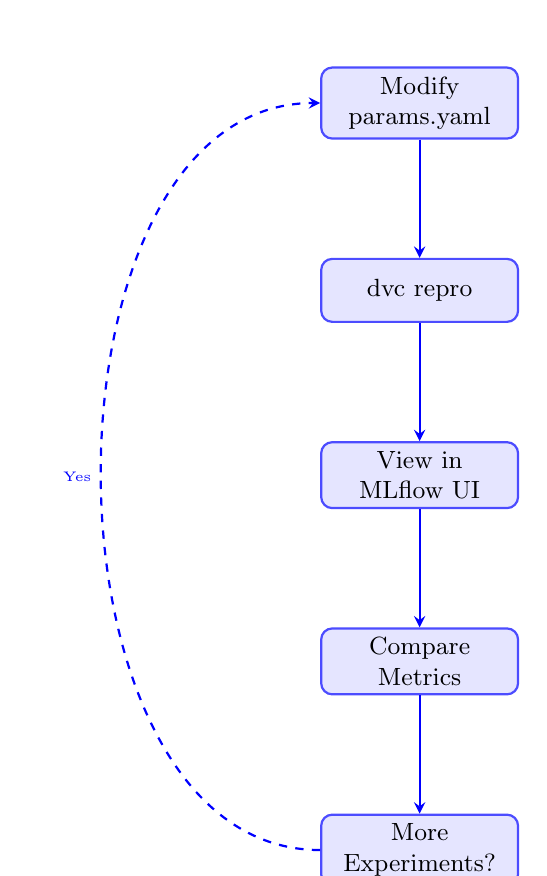
\begin{tikzpicture}[
    node distance=1.5cm,
    box/.style={rectangle, rounded corners, draw=blue!70, fill=blue!10, thick, minimum width=2.5cm, minimum height=0.8cm, align=center, font=\small},
    arrow/.style={->, >=stealth, thick, blue}
]

\node[box] (params) {Modify\\params.yaml};
\node[box, below=of params] (repro) {dvc repro};
\node[box, below=of repro] (mlflow) {View in\\MLflow UI};
\node[box, below=of mlflow] (compare) {Compare\\Metrics};
\node[box, below=of compare] (decide) {More\\Experiments?};

\draw[arrow] (params) -- (repro);
\draw[arrow] (repro) -- (mlflow);
\draw[arrow] (mlflow) -- (compare);
\draw[arrow] (compare) -- (decide);
\draw[arrow, dashed] (decide) to[out=180, in=180] node[left, font=\tiny] {Yes} (params);

\end{tikzpicture}
\end{center}

\subsection{Running Experiment Variations}

\subsubsection{Experiment 1: Initial Configuration}

\begin{lstlisting}[style=yamlstyle]
# params.yaml - Run 1
data_ingestion:
  test_size: 0.25

feature_engineering:
  max_features: 35

model_building:
  n_estimators: 22
  random_state: 2
  max_depth: 11
\end{lstlisting}

\begin{cmdbox}
\begin{verbatim}
dvc repro
\end{verbatim}
\end{cmdbox}

\subsubsection{Experiment 2: Fewer Trees}

\begin{lstlisting}[style=yamlstyle]
# params.yaml - Run 2
data_ingestion:
  test_size: 0.25

feature_engineering:
  max_features: 35

model_building:
  n_estimators: 18    # Changed
  random_state: 2
  max_depth: 5        # Changed
\end{lstlisting}

\begin{cmdbox}
\begin{verbatim}
dvc repro
\end{verbatim}
\end{cmdbox}

\subsubsection{Experiment 3: More Features}

\begin{lstlisting}[style=yamlstyle]
# params.yaml - Run 3
data_ingestion:
  test_size: 0.25

feature_engineering:
  max_features: 50    # Changed

model_building:
  n_estimators: 22
  random_state: 2
  max_depth: 11
\end{lstlisting}

\begin{cmdbox}
\begin{verbatim}
dvc repro
\end{verbatim}
\end{cmdbox}

\subsubsection{Experiment 4: Different Split}

\begin{lstlisting}[style=yamlstyle]
# params.yaml - Run 4
data_ingestion:
  test_size: 0.20     # Changed

feature_engineering:
  max_features: 35

model_building:
  n_estimators: 30    # Changed
  random_state: 2
  max_depth: 15       # Changed
\end{lstlisting}

\begin{cmdbox}
\begin{verbatim}
dvc repro
\end{verbatim}
\end{cmdbox}

\subsubsection{Experiment 5: Balanced Configuration}

\begin{lstlisting}[style=yamlstyle]
# params.yaml - Run 5
data_ingestion:
  test_size: 0.25

feature_engineering:
  max_features: 40    # Changed

model_building:
  n_estimators: 25    # Changed
  random_state: 2
  max_depth: 12       # Changed
\end{lstlisting}

\begin{cmdbox}
\begin{verbatim}
dvc repro
\end{verbatim}
\end{cmdbox}

\newpage

% ========================
% SECTION 9: EXPERIMENT COMPARISON
% ========================
\section{Step 18: Analyzing Experiments in MLflow}

\subsection{Accessing the MLflow UI}

Navigate to your DagShub MLflow tracking URI:

\begin{cmdbox}
\begin{verbatim}
https://dagshub.com/Error-Makes-Clever/
    MLOPS-Dagshub-DVC-Git-Project.mlflow
\end{verbatim}
\end{cmdbox}

\subsection{Experiment Results Summary}

\begin{center}
\begin{tabular}{|l|c|c|c|c|}
\hline
\textbf{Run} & \textbf{AUC} & \textbf{Accuracy} & \textbf{Precision} & \textbf{Recall} \\
\hline
Run 1 (able-ray-853) & 0.9187 & 0.9378 & 0.8302 & 0.6947 \\
\hline
Run 2 (handsome-asp-382) & 0.8656 & 0.8919 & 0.8776 & 0.2756 \\
\hline
Run 3 (placid-gnu-625) & 0.8846 & 0.8922 & 0.8704 & 0.2765 \\
\hline
Run 4 (wise-elk-465) & 0.8994 & 0.9254 & 0.7933 & 0.6263 \\
\hline
Run 5 (receptive-crow-130) & 0.9178 & 0.9334 & 0.8414 & 0.6421 \\
\hline
\end{tabular}
\end{center}

\subsection{Detailed Run Analysis}

\subsubsection{Run 1: able-ray-853}

\begin{infobox}{Run 1 Metrics}
\textbf{Performance}:
\begin{itemize}[leftmargin=*]
    \item AUC: 0.9187
    \item Accuracy: 0.9378
    \item Precision: 0.8302
    \item Recall: 0.6947
\end{itemize}

\textbf{Parameters}:
\begin{itemize}[leftmargin=*]
    \item n\_estimators: 22
    \item max\_depth: 11
    \item max\_features: 35
    \item test\_size: 0.25
\end{itemize}

\textbf{Analysis}: Best overall performance with highest AUC and accuracy.
\end{infobox}

\subsubsection{Run 2: handsome-asp-382}

\begin{infobox}{Run 2 Metrics}
\textbf{Performance}:
\begin{itemize}[leftmargin=*]
    \item AUC: 0.8656
    \item Accuracy: 0.8919
    \item Precision: 0.8776
    \item Recall: 0.2756
\end{itemize}

\textbf{Parameters}:
\begin{itemize}[leftmargin=*]
    \item n\_estimators: 18
    \item max\_depth: 5
    \item max\_features: 35
    \item test\_size: 0.25
\end{itemize}

\textbf{Analysis}: High precision but very low recall. Model is too conservative.
\end{infobox}

\subsubsection{Run 5: receptive-crow-130}

\begin{infobox}{Run 5 Metrics}
\textbf{Performance}:
\begin{itemize}[leftmargin=*]
    \item AUC: 0.9178
    \item Accuracy: 0.9334
    \item Precision: 0.8414
    \item Recall: 0.6421
\end{itemize}

\textbf{Parameters}:
\begin{itemize}[leftmargin=*]
    \item n\_estimators: 25
    \item max\_depth: 12
    \item max\_features: 40
    \item test\_size: 0.25
\end{itemize}

\textbf{Analysis}: Second-best performance, close to Run 1.
\end{infobox}

\newpage

% ========================
% SECTION 10: SELECTING BEST MODEL
% ========================
\section{Step 19: Deciding What "Best" Means}

\subsection{Defining Success Criteria}

Before committing anything, define one primary metric based on your use case:

\begin{center}
\begin{tabular}{|p{0.3\textwidth}|p{0.6\textwidth}|}
\hline
\textbf{Metric Priority} & \textbf{Use Case} \\
\hline
\textbf{Recall} & Spam detection - catch all spam (few false negatives) \\
\hline
\textbf{Precision} & Medical diagnosis - avoid false positives \\
\hline
\textbf{Accuracy} & General classification with balanced classes \\
\hline
\textbf{AUC} & Ranking, threshold tuning, imbalanced data \\
\hline
\textbf{F1-Score} & Balance between precision and recall \\
\hline
\end{tabular}
\end{center}

\subsection{Analysis for Spam Classification}

For spam detection, we typically want:
\begin{enumerate}[leftmargin=*]
    \item High AUC (good separation between classes)
    \item High accuracy (overall correctness)
    \item Balanced precision and recall
\end{enumerate}

\subsection{Ranking the Runs}

\begin{center}
\begin{tabular}{|l|c|c|c|}
\hline
\textbf{Run} & \textbf{AUC} & \textbf{Accuracy} & \textbf{Recommendation} \\
\hline
Run 1 & 0.9187 & 0.9378 & \textbf{Winner} ✓ \\
\hline
Run 5 & 0.9178 & 0.9334 & Runner-up \\
\hline
Run 4 & 0.8994 & 0.9254 & Good \\
\hline
Run 3 & 0.8846 & 0.8922 & Acceptable \\
\hline
Run 2 & 0.8656 & 0.8919 & Poor recall \\
\hline
\end{tabular}
\end{center}

\begin{notebox}
\textbf{Winner: Run 1 (able-ray-853)}

\vspace{0.5em}

\textbf{Justification}:
\begin{itemize}[leftmargin=*]
    \item Highest AUC (0.9187) - best class separation
    \item Highest accuracy (0.9378) - best overall performance
    \item Balanced precision (0.8302) and recall (0.6947)
    \item Reliable and reproducible
\end{itemize}
\end{notebox}

\newpage

% ========================
% SECTION 11: FREEZING BEST MODEL
% ========================
\section{Step 20: Re-creating the Winning Run}

\subsection{Why Re-create?}

\begin{warningbox}
\textbf{Critical MLOps Principle}:

\vspace{0.5em}

Earlier runs were \textbf{exploratory}. Now you are making a \textbf{decision}.

\vspace{0.5em}

\textbf{Why re-create}:
\begin{itemize}[leftmargin=*]
    \item Makes the decision explicit
    \item Creates a clean Git commit representing the approved model
    \item Enables future rollback to this exact state
    \item Documents which experiment was promoted to production
\end{itemize}

\textbf{Don't skip this step!} It's the difference between "I ran some experiments" and "This is our production model."
\end{warningbox}

\subsection{Obtaining Winning Parameters}

Go to MLflow UI → Click on Run 1 (able-ray-853) → View Parameters:

\begin{center}
\begin{tabular}{|l|c|}
\hline
\textbf{Parameter} & \textbf{Value} \\
\hline
test\_size & 0.25 \\
\hline
n\_estimators & 22 \\
\hline
random\_state & 2 \\
\hline
max\_depth & 11 \\
\hline
max\_features & 35 \\
\hline
\end{tabular}
\end{center}

\subsection{Step 21: Update params.yaml}

\begin{examplebox}{params.yaml - Winning Configuration}
\begin{lstlisting}[style=yamlstyle]
data_ingestion:
  test_size: 0.25

feature_engineering:
  max_features: 35

model_building:
  n_estimators: 22
  random_state: 2
  max_depth: 11
\end{lstlisting}
\end{examplebox}

\subsection{Step 22: Run Pipeline with Winning Parameters}

\begin{cmdbox}
\begin{verbatim}
dvc repro
\end{verbatim}
\end{cmdbox}

\textbf{Expected Output}:
\begin{verbatim}
Stage 'data_ingestion' didn't change, skipping
Stage 'data_preprocessing' didn't change, skipping
Stage 'feature_engineering' didn't change, skipping
Stage 'model_building' is cached - skipping run, 
    checking out outputs
Updating lock file 'dvc.lock'

Stage 'model_evaluation' is cached - skipping run, 
    checking out outputs
Updating lock file 'dvc.lock'

To track the changes with git, run:
    git add dvc.lock

To enable auto staging, run:
    dvc config core.autostage true

Use `dvc push` to send your updates to remote storage.
\end{verbatim}

\begin{infobox}{Why No New MLflow Run?}
\textbf{DVC detected that}:
\begin{itemize}[leftmargin=*]
    \item Code did not change
    \item Parameters did not change
    \item Data did not change
\end{itemize}

\textbf{Result}: DVC used cached outputs. No new execution = no new MLflow run.

\vspace{0.5em}

\textbf{This is correct behavior!} We're verifying the winning configuration, not running a new experiment.
\end{infobox}

\subsection{Step 23: Verify Metrics (Sanity Check)}

\begin{cmdbox}
\begin{verbatim}
# Check metrics.json
cat reports/metrics.json
\end{verbatim}
\end{cmdbox}

\textbf{Expected Content}:
\begin{verbatim}
{
    "accuracy": 0.9378200438917337,
    "precision": 0.8301886792452831,
    "recall": 0.6947368421052632,
    "auc": 0.9186759379331932
}
\end{verbatim}

\begin{notebox}
\textbf{Verification}:
\begin{itemize}[leftmargin=*]
    \item Metrics match (or are very close to) Run 1
    \item No accidental changes
    \item Configuration is reproducible
\end{itemize}

If metrics differ wildly → check random seed and data consistency.
\end{notebox}

\newpage

% ========================
% SECTION 12: COMMITTING DECISION
% ========================
\section{Step 24: The Critical Commit}

\subsection{Why This Commit Matters}

\begin{infobox}{The Freezing Commit}
This is the \textbf{most important commit} in your MLOps workflow.

\vspace{0.5em}

\textbf{What this commit represents}:
\begin{itemize}[leftmargin=*]
    \item ✓ This model is \textbf{approved}
    \item ✓ This state is \textbf{reproducible}
    \item ✓ This is \textbf{rollback-safe}
    \item ✓ This is \textbf{deployable}
\end{itemize}

\textbf{What gets committed}:
\begin{itemize}[leftmargin=*]
    \item Code (src/)
    \item Pipeline definition (dvc.yaml)
    \item Parameters (params.yaml)
    \item Lock file (dvc.lock) - contains exact data/model versions
\end{itemize}

\textbf{What does NOT get committed}:
\begin{itemize}[leftmargin=*]
    \item Data files (tracked by DVC)
    \item Model files (tracked by DVC)
    \item Logs
\end{itemize}
\end{infobox}

\subsection{Check Git Status}

\begin{cmdbox}
\begin{verbatim}
git status
\end{verbatim}
\end{cmdbox}

\textbf{Expected Output}:
\begin{verbatim}
On branch main
Your branch is up to date with 'origin/main'.

Changes not staged for commit:
  (use "git add <file>..." to update what will be committed)
  (use "git restore <file>..." to discard changes)
        modified:   .dvc/config
        modified:   dvc.yaml
        modified:   requirements.txt
        modified:   src/Model_Evaluation_Rf.py

Untracked files:
  (use "git add <file>..." to include in what will be committed)
        dvc.lock
        logs/

no changes added to commit
\end{verbatim}

\subsection{Stage and Commit}

\begin{cmdbox}
\begin{verbatim}
# Stage all changes
git add .

# Commit with descriptive message
git commit -m "Freeze best RF model (AUC=0.918, accuracy=0.937)"

# Push to remote
git push origin main
\end{verbatim}
\end{cmdbox}

\subsection{What This Commit Means}

\begin{center}
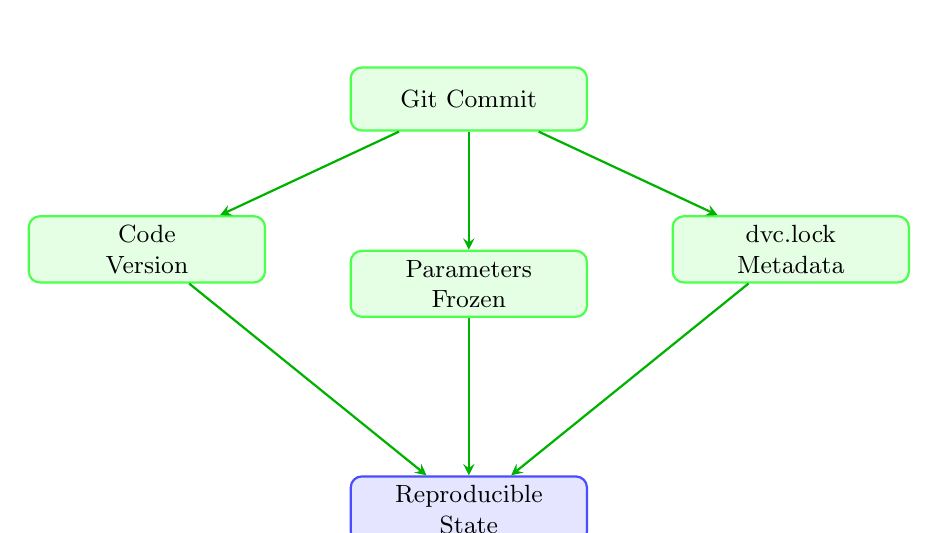
\begin{tikzpicture}[
    node distance=1.5cm,
    box/.style={rectangle, rounded corners, draw=green!70, fill=green!10, thick, minimum width=3cm, minimum height=0.8cm, align=center, font=\small},
    arrow/.style={->, >=stealth, thick, green!70!black}
]

\node[box] (commit) {Git Commit};
\node[box, below left=of commit] (code) {Code\\Version};
\node[box, below=of commit] (params) {Parameters\\Frozen};
\node[box, below right=of commit] (metadata) {dvc.lock\\Metadata};

\draw[arrow] (commit) -- (code);
\draw[arrow] (commit) -- (params);
\draw[arrow] (commit) -- (metadata);

\node[box, below=2cm of params, fill=blue!10, draw=blue!70] (result) {Reproducible\\State};

\draw[arrow] (code) -- (result);
\draw[arrow] (params) -- (result);
\draw[arrow] (metadata) -- (result);

\end{tikzpicture}
\end{center}

\newpage

% ========================
% SECTION 13: PUSHING ARTIFACTS
% ========================
\section{Step 25: Push Data and Model to DVC Remote}

\subsection{Why Push to DVC Remote?}

\begin{warningbox}
\textbf{Git vs DVC Storage}:

\vspace{0.5em}

\textbf{What Git has}:
\begin{itemize}[leftmargin=*]
    \item Code
    \item dvc.lock (metadata with hashes)
    \item Parameters
\end{itemize}

\textbf{What Git does NOT have}:
\begin{itemize}[leftmargin=*]
    \item Actual data files
    \item Actual model files
\end{itemize}

\textbf{Problem}: Without \texttt{dvc push}, teammates cannot reproduce your work!
\end{warningbox}

\subsection{Execute DVC Push}

\begin{cmdbox}
\begin{verbatim}
dvc push
\end{verbatim}
\end{cmdbox}

\textbf{Expected Output}:
\begin{verbatim}
Collecting                           |8.00 [00:00, 2.50entry/s]
Pushing                              |8.00 [00:02, 3.20file/s]
8 files pushed
\end{verbatim}

\subsection{What Gets Pushed}

\begin{center}
\begin{tabular}{|p{0.4\textwidth}|p{0.5\textwidth}|}
\hline
\textbf{Local Location} & \textbf{DVC Remote (S3)} \\
\hline
data/raw/ & Uploaded to S3/ \\
\hline
data/interim/ & Uploaded to S3/ \\
\hline
data/processed/ & Uploaded to S3/ \\
\hline
models/model\_rf.pkl & Uploaded to S3/ \\
\hline
reports/metrics.json & Uploaded to S3/ \\
\hline
\end{tabular}
\end{center}

\subsection{Verification}

\begin{cmdbox}
\begin{verbatim}
# Check S3 directory
ls S3/

# Should see hash-named directories
\end{verbatim}
\end{cmdbox}

\begin{infobox}{Complete State Now}
\textbf{GitHub has}:
\begin{itemize}[leftmargin=*]
    \item Code (src/)
    \item Pipeline (dvc.yaml)
    \item Parameters (params.yaml)
    \item Metadata (dvc.lock)
\end{itemize}

\textbf{DVC Remote (S3) has}:
\begin{itemize}[leftmargin=*]
    \item All data versions
    \item All model versions
    \item All reports
\end{itemize}

\textbf{Result}: Complete reproducibility ✓
\end{infobox}

\newpage

% ========================
% SECTION 14: TAGGING RUNS
% ========================
\section{Step 26: Linking Git Commits to MLflow Runs}

\subsection{Why Tag MLflow Runs?}

\begin{infobox}{The Problem}
\textbf{Situation}:
\begin{itemize}[leftmargin=*]
    \item You have 5 MLflow runs
    \item You committed Run 1 as the winner
    \item Weeks later: "Which MLflow run is our production model?"
\end{itemize}

\textbf{Solution}: Tag the MLflow run with the Git commit hash!

\vspace{0.5em}

\textbf{Benefit}:
\begin{itemize}[leftmargin=*]
    \item Clear link between MLflow experiment and Git commit
    \item Easy to identify production model
    \item Audit trail for compliance
\end{itemize}
\end{infobox}

\subsection{Create Tagging Script}

\begin{examplebox}{Adding\_tag\_to\_runs.py}
\begin{lstlisting}[language=Python]
import subprocess
import mlflow
from mlflow.tracking import MlflowClient
import dagshub

# Authenticate with DagShub
dagshub.init(
    repo_owner="Error-Makes-Clever",
    repo_name="MLOPS-Dagshub-DVC-Git-Project",
    mlflow=True
)

# Set tracking URI
mlflow.set_tracking_uri(
    "https://dagshub.com/Error-Makes-Clever/"
    "MLOPS-Dagshub-DVC-Git-Project.mlflow"
)

# Initialize MLflow client
client = MlflowClient()

# Run ID from MLflow UI (Run 1)
run_id = "eaa2537460244123bc672bee9c22da05"

# Get current Git commit hash
commit = subprocess.check_output(
    ["git", "rev-parse", "HEAD"]
).decode().strip()

# Add tag to MLflow run
client.set_tag(run_id, "git_commit", commit)

# Optional: Add more tags
client.set_tag(run_id, "status", "production")
client.set_tag(run_id, "approved_by", "data_science_team")
client.set_tag(run_id, "deployment_date", "2025-12-20")

print(f"Tags successfully added to run {run_id}")
print(f"   Git commit: {commit}")
\end{lstlisting}
\end{examplebox}

\subsection{Understanding the Script}

\subsubsection{Key Components}

\begin{enumerate}[leftmargin=*]
    \item \textbf{Get Git Commit Hash}:
    \begin{lstlisting}[language=Python]
commit = subprocess.check_output(
    ["git", "rev-parse", "HEAD"]
).decode().strip()
    \end{lstlisting}
    
    \item \textbf{Set Tag in MLflow}:
    \begin{lstlisting}[language=Python]
client.set_tag(run_id, "git_commit", commit)
    \end{lstlisting}
    
    \item \textbf{Additional Metadata Tags}:
    \begin{lstlisting}[language=Python]
client.set_tag(run_id, "status", "production")
client.set_tag(run_id, "approved_by", "team_name")
    \end{lstlisting}
\end{enumerate}

\subsection{Finding the Run ID}

\textbf{Option 1: From MLflow UI}:
\begin{enumerate}[leftmargin=*]
    \item Go to DagShub MLflow interface
    \item Click on Run 1 (able-ray-853)
    \item Copy the Run ID from URL or run details
\end{enumerate}

\textbf{Option 2: From Console Output}:
\begin{verbatim}
View run at: .../runs/eaa2537460244123bc672bee9c22da05
                      ^^^^^^^^^^^^^^^^^^^^^^^^^^^^^^^^^
                      This is the Run ID
\end{verbatim}

\subsection{Step 27: Execute Tagging Script}

\begin{cmdbox}
\begin{verbatim}
python Adding_tag_to_runs.py
\end{verbatim}
\end{cmdbox}

\textbf{Expected Output}:
\begin{verbatim}
Tags successfully added to run eaa2537460244123bc672bee9c22da05
   Git commit: a3f8e2c9d1b4e5f6g7h8i9j0k1l2m3n4
\end{verbatim}

\subsection{Step 28: Verify Tags in MLflow UI}

\begin{enumerate}[leftmargin=*]
    \item Go to MLflow UI
    \item Click on Run 1 (able-ray-853)
    \item Scroll to "Tags" section
    \item Verify tags appear:
\end{enumerate}

\begin{center}
\begin{tabular}{|l|l|}
\hline
\textbf{Tag Key} & \textbf{Tag Value} \\
\hline
git\_commit & a3f8e2c9d1b4e5f6... \\
\hline
status & production \\
\hline
approved\_by & data\_science\_team \\
\hline
deployment\_date & 2025-12-20 \\
\hline
\end{tabular}
\end{center}

\begin{notebox}
\textbf{Best Practice}: Always tag production runs with:
\begin{itemize}[leftmargin=*]
    \item Git commit hash
    \item Deployment status
    \item Approval information
    \item Date/time of promotion
\end{itemize}

This creates a complete audit trail for compliance and debugging.
\end{notebox}

\newpage

% ========================
% SECTION 15: TEAM COLLABORATION
% ========================
\section{Step 29: Multi-Model Experimentation}

\subsection{Scenario: Team with Multiple Models}

\begin{infobox}{Real-World Team Setup}
\textbf{Scenario}:
\begin{itemize}[leftmargin=*]
    \item Data Scientist A: Working on RandomForest
    \item Data Scientist B: Working on XGBoost
    \item Data Scientist C: Working on Neural Networks
\end{itemize}

\textbf{Goal}: Everyone shares the same infrastructure but tracks separate experiments.
\end{infobox}

\subsection{Using Different Experiment Names}

\subsubsection{RandomForest Experiments}

\begin{lstlisting}[language=Python]
# src/Model_Evaluation_Rf.py
mlflow.set_experiment("MLOPS-Project-with-Random-Forest")
\end{lstlisting}

\subsubsection{XGBoost Experiments}

\begin{lstlisting}[language=Python]
# src/Model_Evaluation_Xgb.py
mlflow.set_experiment("MLOPS-Project-with-XGBoost")
\end{lstlisting}

\subsubsection{Neural Network Experiments}

\begin{lstlisting}[language=Python]
# src/Model_Evaluation_NN.py
mlflow.set_experiment("MLOPS-Project-with-Neural-Networks")
\end{lstlisting}

\subsection{Benefits of Separate Experiments}

\begin{enumerate}[leftmargin=*]
    \item \textbf{Organization}: Experiments grouped by model type
    \item \textbf{Clear Ownership}: Each team member manages their experiment
    \item \textbf{Easy Comparison}: Compare within model family first
    \item \textbf{Scalability}: Add new model types without conflicts
\end{enumerate}

\subsection{Viewing All Experiments}

In the DagShub MLflow UI:

\begin{center}
\begin{tabular}{|l|c|c|}
\hline
\textbf{Experiment} & \textbf{Runs} & \textbf{Owner} \\
\hline
MLOPS-Project-with-Random-Forest & 5 & Data Scientist A \\
\hline
MLOPS-Project-with-XGBoost & 8 & Data Scientist B \\
\hline
MLOPS-Project-with-Neural-Networks & 12 & Data Scientist C \\
\hline
\end{tabular}
\end{center}

\begin{notebox}
\textbf{Key Advantage}:

Everyone in your team can:
\begin{itemize}[leftmargin=*]
    \item See all experiments
    \item Compare across models
    \item Learn from each other's work
    \item Avoid duplicate efforts
\end{itemize}

This is impossible with local-only experiment tracking!
\end{notebox}

\newpage

% ========================
% SECTION 16: REPRODUCIBILITY
% ========================
\section{Reproducing the Project on a New Machine}

\subsection{The Reproducibility Challenge}

\begin{warningbox}
\textbf{Common Scenario}:

\vspace{0.5em}

A new team member joins or you need to reproduce the model on a production server.

\vspace{0.5em}

\textbf{Requirements}:
\begin{itemize}[leftmargin=*]
    \item Exact code version
    \item Exact data version
    \item Exact model version
    \item Same environment
\end{itemize}

\textbf{Solution}: Git + DVC + proper setup
\end{warningbox}

\subsection{Important Note About Local DVC Remote}

\begin{infobox}{Critical: Local S3 Directory Limitation}
In this project, the DVC remote is configured as a \textbf{local directory}:

\begin{verbatim}
S3/  (located at: S:\MLOPS-Dagshub-DVC-Git-Project\S3)
\end{verbatim}

\textbf{Problem}: This is a local path, NOT accessible from other machines!

\vspace{0.5em}

\textbf{Options for Team Sharing}:
\begin{enumerate}[leftmargin=*]
    \item Place S3 folder on \textbf{shared network drive}
    \item Use \textbf{NAS / file server}
    \item Map the \textbf{same path on all machines} (e.g., Z:\textbackslash Shared\textbackslash S3)
    \item \textbf{Replace with real cloud remote} (AWS S3, GCS, Azure Blob)
\end{enumerate}

\textbf{Important}: If S3 directory is NOT accessible, \texttt{dvc pull} will fail!
\end{infobox}

\subsection{Reproduction Workflow}

\begin{center}
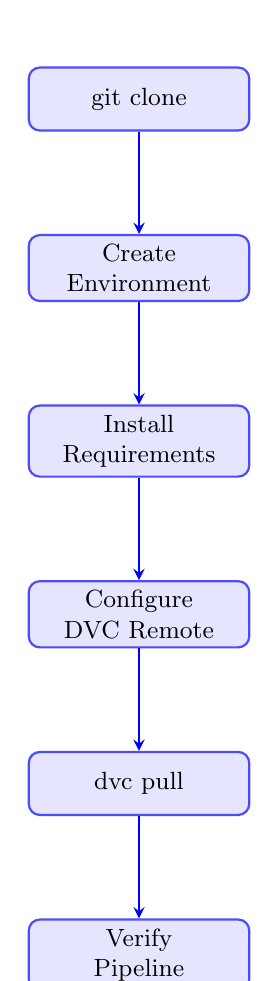
\begin{tikzpicture}[
    node distance=1.3cm,
    box/.style={rectangle, rounded corners, draw=blue!70, fill=blue!10, thick, minimum width=2.8cm, minimum height=0.8cm, align=center, font=\small},
    arrow/.style={->, >=stealth, thick, blue}
]

\node[box] (clone) {git clone};
\node[box, below=of clone] (env) {Create\\Environment};
\node[box, below=of env] (install) {Install\\Requirements};
\node[box, below=of install] (remote) {Configure\\DVC Remote};
\node[box, below=of remote] (pull) {dvc pull};
\node[box, below=of pull] (verify) {Verify\\Pipeline};

\draw[arrow] (clone) -- (env);
\draw[arrow] (env) -- (install);
\draw[arrow] (install) -- (remote);
\draw[arrow] (remote) -- (pull);
\draw[arrow] (pull) -- (verify);

\end{tikzpicture}
\end{center}

\subsection{Step-by-Step Reproduction}

\subsubsection{Step 1: Clone Repository}

\begin{cmdbox}
\begin{verbatim}
# Clone Git repository
git clone https://github.com/Error-Makes-Clever/
    MLOPS-Dagshub-DVC-Git-Project.git

cd MLOPS-Dagshub-DVC-Git-Project
\end{verbatim}
\end{cmdbox}

\textbf{What this does}:
\begin{itemize}[leftmargin=*]
    \item Downloads all code files
    \item Downloads dvc.yaml (pipeline definition)
    \item Downloads dvc.lock (file version metadata)
    \item Downloads params.yaml (hyperparameters)
    \item Does NOT download data/models (DVC handles this)
\end{itemize}

\subsubsection{Step 2: Create and Activate Environment}

\begin{cmdbox}
\begin{verbatim}
# Create virtual environment
python -m venv venv

# Activate (Windows)
venv\Scripts\activate

# Activate (Linux/Mac)
source venv/bin/activate
\end{verbatim}
\end{cmdbox}

\textbf{Verify activation}:
\begin{cmdbox}
\begin{verbatim}
# Check Python path (should point to venv)
which python    # Linux/Mac
where python    # Windows
\end{verbatim}
\end{cmdbox}

\subsubsection{Step 3: Install Requirements}

\begin{cmdbox}
\begin{verbatim}
pip install -r requirements.txt
\end{verbatim}
\end{cmdbox}

\textbf{Expected packages}:
\begin{itemize}[leftmargin=*]
    \item dvc
    \item numpy, pandas
    \item matplotlib, wordcloud
    \item nltk
    \item scikit-learn
    \item xgboost
    \item pyyaml
    \item mlflow
    \item dagshub
\end{itemize}

\textbf{Verify installation}:
\begin{cmdbox}
\begin{verbatim}
# Check installed packages
pip list

# Verify DVC
dvc version

# Verify MLflow
mlflow --version
\end{verbatim}
\end{cmdbox}

\subsubsection{Step 4: Configure DVC Remote Access}

\begin{cmdbox}
\begin{verbatim}
# Check current remote configuration
dvc remote list
\end{verbatim}
\end{cmdbox}

\textbf{Expected Output}:
\begin{verbatim}
dvc_origin    S3
\end{verbatim}

\begin{notebox}
\textbf{Understanding the Remote Path}:

The remote path in the repository is relative (\texttt{S3}), which means it expects the S3 folder to be in the same parent directory as the project.

\vspace{0.5em}

\textbf{Original setup}:
\begin{verbatim}
S:\MLOPS-Dagshub-DVC-Git-Project\
    ├── S3/                    (DVC remote)
    └── project/               (Git repository)
\end{verbatim}

\textbf{For reproduction}: You need to ensure the S3 directory is accessible at the same relative location OR update the remote URL.
\end{notebox}

\textbf{If path needs updating}:

\begin{examplebox}{Update DVC Remote Path}
\begin{lstlisting}[style=bashstyle]
# Option 1: Use shared network drive (Windows)
dvc remote modify dvc_origin url Z:\Shared\MLOPS\S3

# Option 2: Use UNC path (Windows)
dvc remote modify dvc_origin url \\server\share\S3

# Option 3: Use mounted path (Linux/Mac)
dvc remote modify dvc_origin url /mnt/shared/S3

# Option 4: Use absolute local path
dvc remote modify dvc_origin url /path/to/shared/S3

# Verify updated configuration
dvc remote list -v
\end{lstlisting}
\end{examplebox}

\textbf{Check .dvc/config after modification}:
\begin{cmdbox}
\begin{verbatim}
cat .dvc/config
\end{verbatim}
\end{cmdbox}

\textbf{Expected content}:
\begin{verbatim}
[core]
    remote = dvc_origin

['remote "dvc_origin"']
    url = /path/to/shared/S3
\end{verbatim}

\subsubsection{Step 5: Pull Data and Models}

\begin{cmdbox}
\begin{verbatim}
dvc pull
\end{verbatim}
\end{cmdbox}

\textbf{Expected Output}:
\begin{verbatim}
Collecting                        |8.00 [00:00, 10.0entry/s]
Fetching
Building workspace index          |8.00 [00:00, 100entry/s]
Comparing indexes                 |8.00 [00:00, 200entry/s]
Applying changes                  |8.00 [00:01, 5.00file/s]
8 files fetched
\end{verbatim}

\textbf{What gets downloaded}:
\begin{itemize}[leftmargin=*]
    \item \texttt{data/raw/train.csv}
    \item \texttt{data/raw/test.csv}
    \item \texttt{data/interim/train\_processed.csv}
    \item \texttt{data/interim/test\_processed.csv}
    \item \texttt{data/processed/train\_tfidf.csv}
    \item \texttt{data/processed/test\_tfidf.csv}
    \item \texttt{models/model\_rf.pkl}
    \item \texttt{reports/metrics.json}
\end{itemize}

\begin{infobox}{How DVC Pull Works}
\textbf{Process}:
\begin{enumerate}[leftmargin=*]
    \item DVC reads \texttt{dvc.lock} to get file hashes
    \item Checks if files exist in local cache (\texttt{.dvc/cache/})
    \item If missing, downloads from remote storage (S3)
    \item Copies files from cache to workspace
    \item Verifies checksums match
\end{enumerate}

\textbf{Result}: Exact same data/models as the original machine!
\end{infobox}

\subsubsection{Step 6: Verify Pipeline Status}

\begin{cmdbox}
\begin{verbatim}
dvc status
\end{verbatim}
\end{cmdbox}

\textbf{Expected Output}:
\begin{verbatim}
Data and pipelines are up to date.
\end{verbatim}

\textbf{If you see changes}:
\begin{verbatim}
data_ingestion:
    changed deps:
        modified:  src/Data_Ingestion.py
\end{verbatim}

\textbf{Possible causes}:
\begin{itemize}[leftmargin=*]
    \item Line ending differences (Windows vs Linux)
    \item Incomplete pull
    \item Local modifications
\end{itemize}

\textbf{Solution}:
\begin{cmdbox}
\begin{verbatim}
# Discard local changes
git checkout .

# Re-pull data
dvc pull

# Check status again
dvc status
\end{verbatim}
\end{cmdbox}

\subsubsection{Step 7 (Optional): Re-run Pipeline}

\begin{cmdbox}
\begin{verbatim}
dvc repro
\end{verbatim}
\end{cmdbox}

\textbf{Expected Result}:
\begin{verbatim}
Stage 'data_ingestion' didn't change, skipping
Stage 'data_preprocessing' didn't change, skipping
Stage 'feature_engineering' didn't change, skipping
Stage 'model_building' is cached - skipping run
Stage 'model_evaluation' is cached - skipping run

Data and pipelines are up to date.
\end{verbatim}

\textbf{What this means}:
\begin{itemize}[leftmargin=*]
    \item All stages are cached (no re-execution)
    \item No new MLflow runs created
    \item Guaranteed reproducibility $\checkmark$
    \item Pipeline is working correctly $\checkmark$
\end{itemize}

\subsection{Verification Checklist}

\begin{center}
\begin{tabular}{|l|c|l|}
\hline
\textbf{Item} & \textbf{Status} & \textbf{Command} \\
\hline
Code matches & $\checkmark$ & \texttt{git log --oneline} \\
\hline
Data matches & $\checkmark$ & \texttt{dvc status} \\
\hline
Model exists & $\checkmark$ & \texttt{ls models/} \\
\hline
Metrics match & $\checkmark$ & \texttt{cat reports/metrics.json} \\
\hline
Environment ready & $\checkmark$ & \texttt{pip list} \\
\hline
Pipeline works & $\checkmark$ & \texttt{dvc repro} \\
\hline
\end{tabular}
\end{center}

\subsection{Manual Verification}

\subsubsection{Verify Metrics}

\begin{cmdbox}
\begin{verbatim}
cat reports/metrics.json
\end{verbatim}
\end{cmdbox}

\textbf{Expected content}:
\begin{verbatim}
{
    "accuracy": 0.9378200438917337,
    "precision": 0.8301886792452831,
    "recall": 0.6947368421052632,
    "auc": 0.9186759379331932
}
\end{verbatim}

\subsubsection{Verify Parameters}

\begin{cmdbox}
\begin{verbatim}
cat params.yaml
\end{verbatim}
\end{cmdbox}

\textbf{Expected content}:
\begin{verbatim}
data_ingestion:
  test_size: 0.25

feature_engineering:
  max_features: 35

model_building:
  n_estimators: 22
  random_state: 2
  max_depth: 11
\end{verbatim}

\subsubsection{Test Model Loading}

\begin{examplebox}{test\_model.py}
\begin{lstlisting}[language=Python]
import pickle
import pandas as pd

# Load model
with open('models/model_rf.pkl', 'rb') as f:
    model = pickle.load(f)

print(f"Model type: {type(model)}")
print(f"Number of estimators: {model.n_estimators}")
print(f"Max depth: {model.max_depth}")

# Load test data
test_data = pd.read_csv('data/processed/test_tfidf.csv')
X_test = test_data.iloc[:, :-1].values
y_test = test_data.iloc[:, -1].values

# Make predictions
predictions = model.predict(X_test)
print(f"Predictions shape: {predictions.shape}")
print(f"First 10 predictions: {predictions[:10]}")

print("\nModel loaded and working correctly!")
\end{lstlisting}
\end{examplebox}

\begin{cmdbox}
\begin{verbatim}
python test_model.py
\end{verbatim}
\end{cmdbox}

\textbf{Expected output}:
\begin{verbatim}
Model type: <class 'sklearn.ensemble._forest.RandomForestClassifier'>
Number of estimators: 22
Max depth: 11
Predictions shape: (1384,)
First 10 predictions: [0 0 0 1 0 0 0 0 0 0]

Model loaded and working correctly!
\end{verbatim}

\subsection{Why This Matters in MLOps}

\begin{infobox}{Reproducibility Benefits}
\textbf{Without dvc pull}:
\begin{itemize}[leftmargin=*]
    \item Data is missing
    \item Models cannot be loaded
    \item Results cannot be verified
    \item Team collaboration breaks
    \item Production deployment fails
\end{itemize}

\textbf{With dvc pull}:
\begin{itemize}[leftmargin=*]
    \item Exact data restored
    \item Approved model retrieved
    \item Everyone works on same version
    \item Perfect reproducibility
    \item Confident deployment
\end{itemize}
\end{infobox}

\subsection{Troubleshooting Reproduction Issues}

\subsubsection{Issue 1: "Remote not found"}

\textbf{Error}:
\begin{verbatim}
ERROR: failed to pull data from the cloud - 
    [Errno 2] No such file or directory: 'S3'
\end{verbatim}

\textbf{Solution}:
\begin{enumerate}[leftmargin=*]
    \item Confirm S3 directory location with team
    \item Update remote URL:
    \begin{cmdbox}
\begin{verbatim}
dvc remote modify dvc_origin url <correct-path>
\end{verbatim}
    \end{cmdbox}
    \item Verify access permissions
    \item Try pulling again
\end{enumerate}

\subsubsection{Issue 2: "Permission denied"}

\textbf{Error}:
\begin{verbatim}
ERROR: failed to pull data - [Errno 13] Permission denied
\end{verbatim}

\textbf{Solution}:
\begin{itemize}[leftmargin=*]
    \item Check read permissions on shared directory
    \item On Linux/Mac: \texttt{ls -la /path/to/S3}
    \item On Windows: Check folder properties → Security tab
    \item Contact IT for network drive access
\end{itemize}

\subsubsection{Issue 3: "Checksum mismatch"}

\textbf{Error}:
\begin{verbatim}
ERROR: checksum mismatch for 'data/raw/train.csv'
\end{verbatim}

\textbf{Solution}:
\begin{cmdbox}
\begin{verbatim}
# Remove corrupted cache
rm -rf .dvc/cache

# Re-pull data
dvc pull
\end{verbatim}
\end{cmdbox}

\subsubsection{Issue 4: "Python package conflicts"}

\textbf{Error}:
\begin{verbatim}
ImportError: cannot import name 'X' from 'Y'
\end{verbatim}

\textbf{Solution}:
\begin{cmdbox}
\begin{verbatim}
# Recreate environment
deactivate
rm -rf venv
python -m venv venv
source venv/bin/activate  # or venv\Scripts\activate

# Reinstall exact versions
pip install -r requirements.txt

# Verify
pip list
\end{verbatim}
\end{cmdbox}

% ========================
% SECTION 17: MENTAL MODEL
% ========================
\section{Complete Mental Model}

\subsection{The Three-System Architecture}

\begin{center}
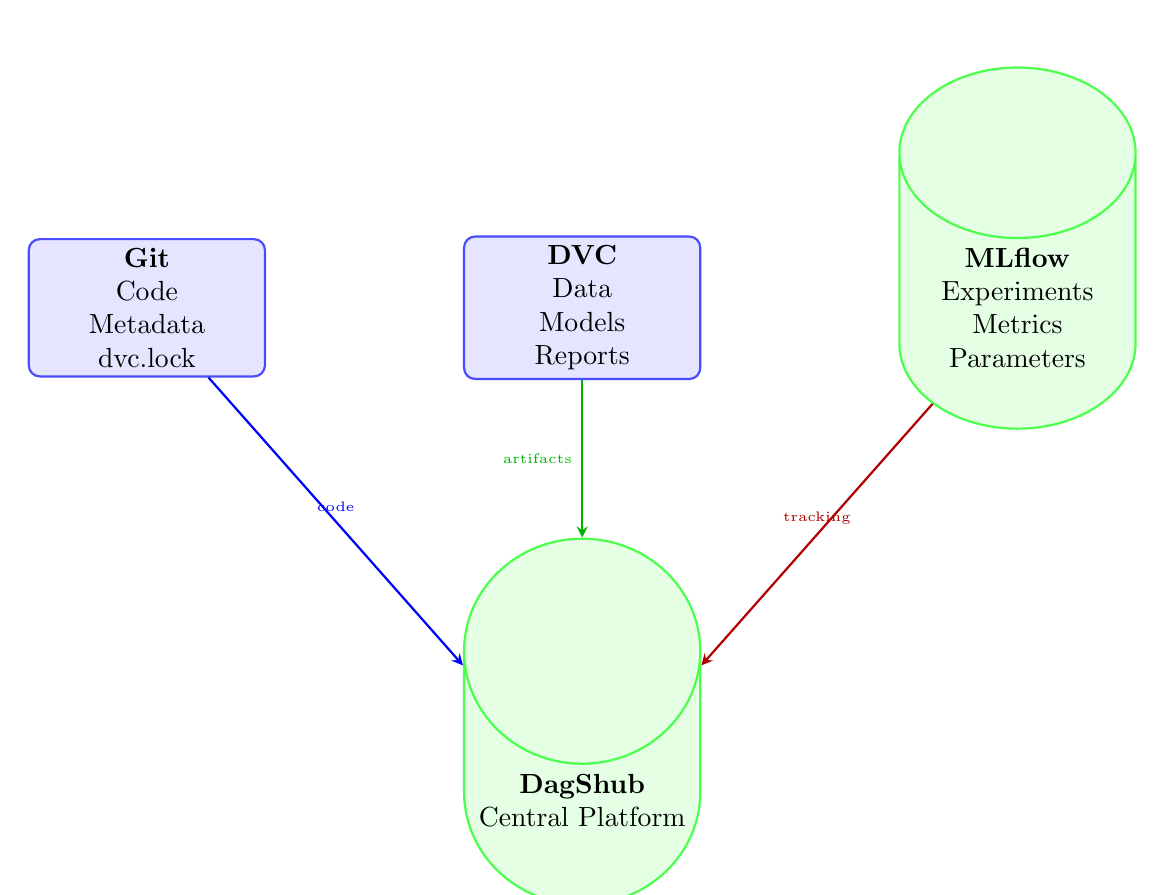
\begin{tikzpicture}[
    node distance=2.5cm,
    box/.style={rectangle, rounded corners, draw=blue!70, fill=blue!10, thick, minimum width=3cm, minimum height=1.5cm, align=center},
    storage/.style={cylinder, shape border rotate=90, draw=green!70, fill=green!10, thick, minimum width=3cm, minimum height=1.5cm, align=center},
    arrow/.style={->, >=stealth, thick}
]

\node[box] (git) {\textbf{Git}\\Code\\Metadata\\dvc.lock};
\node[box, right=of git] (dvc) {\textbf{DVC}\\Data\\Models\\Reports};
\node[storage, right=of dvc] (mlflow) {\textbf{MLflow}\\Experiments\\Metrics\\Parameters};

\node[storage, below=2cm of dvc] (dagshub) {\textbf{DagShub}\\Central Platform};

\draw[arrow, blue] (git) -- node[above, font=\tiny] {code} (dagshub);
\draw[arrow, green!70!black] (dvc) -- node[left, font=\tiny] {artifacts} (dagshub);
\draw[arrow, red!70!black] (mlflow) -- node[above, font=\tiny] {tracking} (dagshub);

\end{tikzpicture}
\end{center}

\subsection{Understanding Each Component}

\subsubsection{Git: Code and Metadata}

\begin{infobox}{Git Responsibilities}
\textbf{What Git tracks}:
\begin{itemize}[leftmargin=*]
    \item Source code (src/)
    \item Pipeline definition (dvc.yaml)
    \item Parameters (params.yaml)
    \item Lock file (dvc.lock) - contains hashes
    \item Configuration files
    \item Documentation (README.md)
\end{itemize}

\textbf{What Git does NOT track}:
\begin{itemize}[leftmargin=*]
    \item Data files (too large)
    \item Model files (binary)
    \item Logs
    \item Cache directories
\end{itemize}

\textbf{Key Commands}:
\begin{itemize}[leftmargin=*]
    \item \texttt{git add .} - Stage changes
    \item \texttt{git commit -m "message"} - Save snapshot
    \item \texttt{git push} - Upload to GitHub
    \item \texttt{git checkout <hash>} - Switch versions
\end{itemize}
\end{infobox}

\subsubsection{DVC: Data and Models}

\begin{infobox}{DVC Responsibilities}
\textbf{What DVC tracks}:
\begin{itemize}[leftmargin=*]
    \item All data versions (raw, processed)
    \item All model versions
    \item Reports and metrics files
    \item Pipeline outputs
\end{itemize}

\textbf{How DVC works}:
\begin{itemize}[leftmargin=*]
    \item Stores actual files in remote storage (S3)
    \item Stores metadata (hashes) in Git (dvc.lock)
    \item Local cache (.dvc/cache/) for speed
    \item Content-addressable storage
\end{itemize}

\textbf{Key Commands}:
\begin{itemize}[leftmargin=*]
    \item \texttt{dvc add <file>} - Track file
    \item \texttt{dvc push} - Upload to remote
    \item \texttt{dvc pull} - Download from remote
    \item \texttt{dvc repro} - Run pipeline
\end{itemize}
\end{infobox}

\subsubsection{MLflow: Experiment Tracking}

\begin{infobox}{MLflow Responsibilities}
\textbf{What MLflow tracks}:
\begin{itemize}[leftmargin=*]
    \item All experiment runs
    \item Metrics (accuracy, precision, etc.)
    \item Parameters (hyperparameters)
    \item Artifacts (optional)
    \item Tags and metadata
\end{itemize}

\textbf{Benefits}:
\begin{itemize}[leftmargin=*]
    \item Visual comparison of experiments
    \item Centralized tracking (team-wide)
    \item Experiment history preserved
    \item Easy metric comparison
\end{itemize}

\textbf{Key Functions}:
\begin{itemize}[leftmargin=*]
    \item \texttt{mlflow.set\_experiment()} - Group runs
    \item \texttt{mlflow.start\_run()} - Begin tracking
    \item \texttt{mlflow.log\_metric()} - Log metric
    \item \texttt{mlflow.log\_param()} - Log parameter
\end{itemize}
\end{infobox}

\subsection{Data Flow Summary}

\begin{center}
\begin{tabular}{|l|p{0.65\textwidth}|}
\hline
\textbf{Command} & \textbf{What Happens} \\
\hline
\texttt{git commit} & Saves code, params.yaml, dvc.lock to Git \\
\hline
\texttt{git push} & Uploads Git commits to GitHub \\
\hline
\texttt{dvc push} & Uploads data/models to DVC remote (S3) \\
\hline
\texttt{dvc pull} & Downloads data/models from DVC remote \\
\hline
\texttt{dvc repro} & Runs pipeline, updates dvc.lock \\
\hline
\texttt{mlflow.log\_*} & Logs metrics/params to MLflow (DagShub) \\
\hline
\texttt{git checkout} & Restores code to specific commit \\
\hline
\end{tabular}
\end{center}

\subsection{Complete Workflow Visualization}

\begin{center}
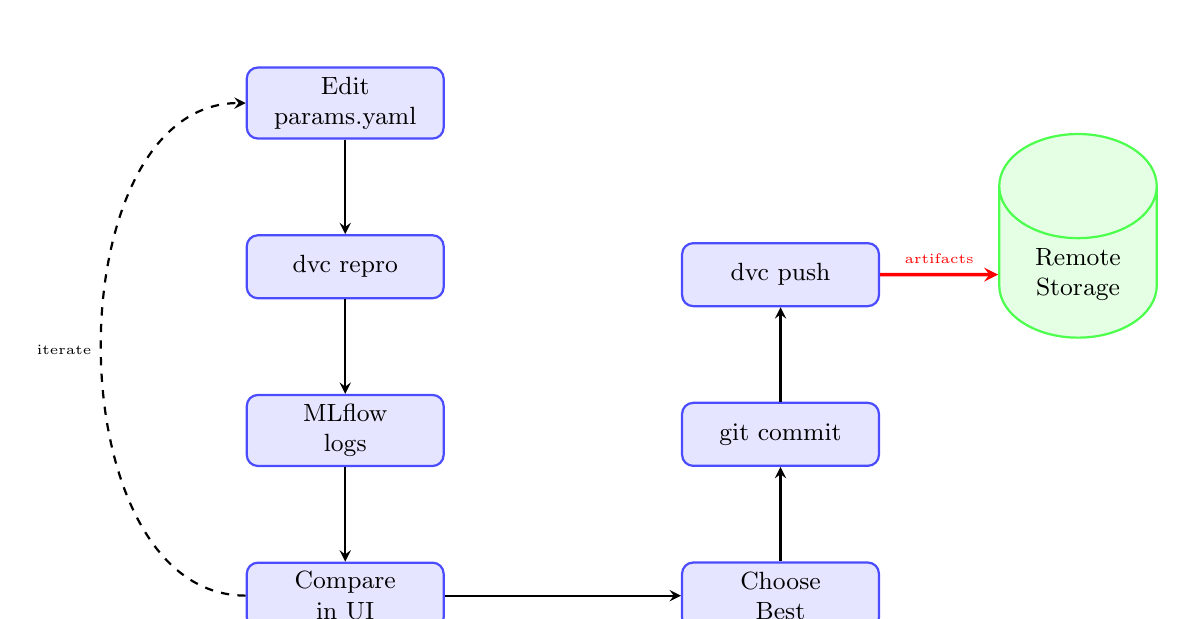
\begin{tikzpicture}[
    node distance=1.2cm,
    box/.style={rectangle, rounded corners, draw=blue!70, fill=blue!10, thick, minimum width=2.5cm, minimum height=0.8cm, align=center, font=\small},
    storage/.style={cylinder, shape border rotate=90, draw=green!70, fill=green!10, thick, minimum width=2cm, minimum height=1cm, align=center, font=\small},
    arrow/.style={->, >=stealth, thick},
    redarrow/.style={->, >=stealth, very thick, red}
]

% Left: Experimentation
\node[box] (params) {Edit\\params.yaml};
\node[box, below=of params] (repro) {dvc repro};
\node[box, below=of repro] (mlflow) {MLflow\\logs};
\node[box, below=of mlflow] (compare) {Compare\\in UI};

% Right: Freezing
\node[box, right=3cm of compare] (decide) {Choose\\Best};
\node[box, above=of decide] (commit) {git commit};
\node[box, above=of commit] (push) {dvc push};
\node[storage, right=1.5cm of push] (storage) {Remote\\Storage};

% Arrows
\draw[arrow] (params) -- (repro);
\draw[arrow] (repro) -- (mlflow);
\draw[arrow] (mlflow) -- (compare);
\draw[arrow] (compare) -- (decide);
\draw[arrow] (decide) -- (commit);
\draw[arrow] (commit) -- (push);
\draw[redarrow] (push) -- node[above, font=\tiny] {artifacts} (storage);
\draw[arrow, dashed] (compare) to[out=180, in=180] node[left, font=\tiny] {iterate} (params);

\end{tikzpicture}
\end{center}

\subsection{Key Concepts Review}

\begin{center}
\begin{tabular}{|p{0.3\textwidth}|p{0.6\textwidth}|}
\hline
\textbf{Concept} & \textbf{Meaning} \\
\hline
\textbf{Experiment} & Collection of related runs (e.g., all RandomForest tests) \\
\hline
\textbf{Run} & Single execution with specific parameters \\
\hline
\textbf{dvc.lock} & File with exact versions (hashes) of all data/models \\
\hline
\textbf{params.yaml} & Configuration file with hyperparameters \\
\hline
\textbf{DVC Remote} & Storage location for data/models (S3, GCS, local) \\
\hline
\textbf{Freezing} & Committing approved model configuration to Git \\
\hline
\textbf{Tagging} & Linking MLflow runs to Git commits \\
\hline
\textbf{Reproducibility} & Ability to recreate exact results on any machine \\
\hline
\end{tabular}
\end{center}

\newpage

% ========================
% SECTION 18: BEST PRACTICES
% ========================
\section{MLOps Best Practices}

\subsection{Experiment Management}

\subsubsection{Naming Conventions}

\begin{examplebox}{Good Experiment Names}
$\checkmark$ "MLOPS-Project-with-Random-Forest"\\
$\checkmark$ "MLOPS-Project-with-XGBoost"\\
$\checkmark$ "MLOPS-Project-with-BERT-Embeddings"\\
$\checkmark$ "Spam-Detection-RandomForest-v2"\\[6 pt]

$\wrongmark$ "experiment1"\\
$\wrongmark$ "test"\\
$\wrongmark$ "my\_experiment"\\
$\wrongmark$ "asdf"
\end{examplebox}

\subsubsection{Commit Message Best Practices}

\begin{examplebox}{Good Commit Messages}
$\checkmark$ Freeze best RF model (AUC=0.918, accuracy=0.937)\\
$\checkmark$ Experiment: increase max\_depth to 15, acc +0.02\\
$\checkmark$ Fix: correct data leakage in preprocessing\\
$\checkmark$ Add: XGBoost baseline (AUC=0.901)\\
$\checkmark$ Refactor: modularize feature engineering\\[6pt]

$\wrongmark $ Update\\
$\wrongmark$ Fix bug\\
$\wrongmark$ Changes\\
$\wrongmark$ WIP\\
$\wrongmark$ temp
\end{examplebox}

\subsubsection{Parameter Documentation}

\begin{lstlisting}[style=yamlstyle]
# params.yaml with comments
data_ingestion:
  test_size: 0.25      # Standard 75/25 split

feature_engineering:
  max_features: 35     # Optimal from grid search

model_building:
  n_estimators: 22     # Best balance: speed vs accuracy
  random_state: 2      # For reproducibility
  max_depth: 11        # Prevents overfitting
\end{lstlisting}

\subsection{DVC Remote Management}

\subsubsection{Production Setup Recommendations}

\begin{warningbox}
\textbf{For Production: Use Cloud Storage}

\vspace{0.5em}

\textbf{Why local directories don't scale}:
\begin{itemize}[leftmargin=*]
    \item Not accessible across team
    \item No disaster recovery
    \item Access control issues
    \item Cannot use in CI/CD pipelines
    \item No versioning/backup
\end{itemize}

\textbf{Recommended Solutions}:
\begin{itemize}[leftmargin=*]
    \item AWS S3 (most popular, cost-effective)
    \item Google Cloud Storage (GCS)
    \item Azure Blob Storage
    \item MinIO (self-hosted S3-compatible)
\end{itemize}
\end{warningbox}

\subsubsection{Migrating to AWS S3}

\begin{examplebox}{AWS S3 Setup}
\begin{lstlisting}[style=bashstyle]
# Install AWS support
pip install dvc[s3] awscli

# Configure AWS credentials
aws configure
# Enter: Access Key ID
# Enter: Secret Access Key
# Enter: Region (e.g., us-east-1)
# Enter: Output format (json)

# Remove local remote
dvc remote remove dvc_origin

# Add S3 remote
dvc remote add -d s3remote s3://my-bucket/dvc-storage

# Verify configuration
dvc remote list

# Push data to S3
dvc push

# Commit updated config
git add .dvc/config
git commit -m "Migrate to AWS S3 remote storage"
git push
\end{lstlisting}
\end{examplebox}

\subsection{MLflow Best Practices}

\subsubsection{What to Log}

\begin{center}
\begin{tabular}{|l|l|}
\hline
\textbf{Always Log} & \textbf{Consider Logging} \\
\hline
Primary metrics (accuracy, AUC) & Training time \\
\hline
All hyperparameters & Memory usage \\
\hline
Data split ratios & Number of features \\
\hline
Random seeds & Data version/hash \\
\hline
Model type & Hardware info (GPU/CPU) \\
\hline
Feature names & Dataset size \\
\hline
\end{tabular}
\end{center}

\subsubsection{Comprehensive Tagging Strategy}

\begin{examplebox}{Complete Tagging Example}
\begin{lstlisting}[language=Python]
from mlflow.tracking import MlflowClient
import subprocess

client = MlflowClient()
run_id = "your-run-id"

# Tag with Git info
commit_hash = subprocess.check_output(
    ["git", "rev-parse", "HEAD"]
).decode().strip()
branch = subprocess.check_output(
    ["git", "rev-parse", "--abbrev-ref", "HEAD"]
).decode().strip()

client.set_tag(run_id, "git_commit", commit_hash)
client.set_tag(run_id, "git_branch", branch)

# Tag with deployment info
client.set_tag(run_id, "status", "production")
client.set_tag(run_id, "environment", "production")

# Tag with approval metadata
client.set_tag(run_id, "approved_by", "john_doe")
client.set_tag(run_id, "approval_date", "2025-12-20")
client.set_tag(run_id, "model_version", "v2.1.0")

# Tag with business context
client.set_tag(run_id, "use_case", "spam_detection")
client.set_tag(run_id, "department", "email_security")
client.set_tag(run_id, "priority", "high")

print(f"All tags added to run {run_id}")
\end{lstlisting}
\end{examplebox}

\subsection{Workflow Best Practices}

\subsubsection{Before Starting Experiments}

\begin{enumerate}[leftmargin=*]
    \item \textbf{Define success criteria}:
    \begin{itemize}
        \item What metric matters most?
        \item What's acceptable performance?
        \item What's the baseline?
    \end{itemize}
    
    \item \textbf{Set baseline}:
    \begin{itemize}
        \item Run simplest model first
        \item Document baseline performance
        \item Use as comparison point
    \end{itemize}
    
    \item \textbf{Document assumptions}:
    \begin{itemize}
        \item Data assumptions
        \item Business constraints
        \item Resource limitations
    \end{itemize}
    
    \item \textbf{Plan experiments}:
    \begin{itemize}
        \item Create experiment matrix
        \item Prioritize high-impact experiments
        \item Estimate time/resources
    \end{itemize}
\end{enumerate}

\subsubsection{During Experimentation}

\begin{enumerate}[leftmargin=*]
    \item \textbf{Change one variable at a time}:
    \begin{itemize}
        \item Isolate effects
        \item Understand what works
        \item Build intuition
    \end{itemize}
    
    \item \textbf{Log everything}:
    \begin{itemize}
        \item All parameters
        \item All metrics
        \item Observations/notes
        \item Unexpected results
    \end{itemize}
    
    \item \textbf{Keep detailed notes}:
    \begin{itemize}
        \item Why you tried something
        \item What you observed
        \item Hypotheses for next steps
    \end{itemize}
    
    \item \textbf{Compare systematically}:
    \begin{itemize}
        \item Use MLflow UI
        \item Create comparison tables
        \item Visualize trends
    \end{itemize}
\end{enumerate}

\subsubsection{After Choosing Best Model}

\begin{enumerate}[leftmargin=*]
    \item \textbf{Verify reproducibility}:
    \begin{itemize}
        \item Run pipeline again
        \item Confirm metrics match
        \item Check random seed
    \end{itemize}
    
    \item \textbf{Document decision}:
    \begin{itemize}
        \item Why this model?
        \item What alternatives considered?
        \item Trade-offs made
    \end{itemize}
    
    \item \textbf{Freeze configuration}:
    \begin{itemize}
        \item Git commit with clear message
        \item Include metrics in message
        \item Tag as milestone
    \end{itemize}
    
    \item \textbf{Push artifacts}:
    \begin{itemize}
        \item \texttt{dvc push} to remote
        \item Verify upload successful
        \item Test pull on different machine
    \end{itemize}
    
    \item \textbf{Tag MLflow run}:
    \begin{itemize}
        \item Link to Git commit
        \item Add production status
        \item Include approval info
    \end{itemize}
    
    \item \textbf{Update documentation}:
    \begin{itemize}
        \item README with latest model info
        \item Wiki with experiment summary
        \item Deployment guide
    \end{itemize}
\end{enumerate}

\subsection{Team Collaboration Guidelines}

\subsubsection{Communication Best Practices}

\begin{itemize}[leftmargin=*]
    \item \textbf{Share experiment plans}: Before starting work
    \item \textbf{Review each other's runs}: Learn together
    \item \textbf{Discuss surprises}: Unexpected results
    \item \textbf{Document learnings}: Wiki or shared docs
    \item \textbf{Regular sync meetings}: Weekly experiment reviews
    \item \textbf{Clear ownership}: Who owns which experiment
    \item \textbf{Celebrate wins}: Share successful experiments
\end{itemize}

\subsubsection{Avoiding Conflicts}

\begin{itemize}[leftmargin=*]
    \item \textbf{Use separate experiments}: One per person/model type
    \item \textbf{Coordinate on shared data}: Don't modify raw data
    \item \textbf{Review before freezing}: Get team approval
    \item \textbf{Clear ownership}: Who decides what to freeze
    \item \textbf{Communicate changes}: Notify team of updates
    \item \textbf{Use branches}: Feature branches for big changes
\end{itemize}

\subsection{Code Quality Best Practices}

\subsubsection{Logging Standards}

\begin{lstlisting}[language=Python]
import logging

# Configure logger
logger = logging.getLogger(__name__)
logger.setLevel('DEBUG')

# Good logging practice
logger.debug('Loading data from %s', file_path)
logger.info('Training started with %d samples', n_samples)
logger.warning('Missing %d features, using defaults', n_missing)
logger.error('Failed to load model: %s', error_msg)

# Bad logging practice
logger.info('Loading data')  # Not informative
print('Training started')    # Should use logger
\end{lstlisting}

\subsubsection{Error Handling}

\begin{lstlisting}[language=Python]
def load_data(file_path: str) -> pd.DataFrame:
    """Load data with comprehensive error handling."""
    try:
        # Attempt operation
        df = pd.read_csv(file_path)
        logger.info(f'Loaded {len(df)} rows from {file_path}')
        return df
        
    except FileNotFoundError:
        logger.error(f'File not found: {file_path}')
        raise
        
    except pd.errors.ParserError as e:
        logger.error(f'Failed to parse CSV: {e}')
        raise
        
    except Exception as e:
        logger.error(f'Unexpected error: {e}')
        raise
\end{lstlisting}

\subsubsection{Type Hints and Documentation}

\begin{lstlisting}[language=Python]
from typing import Tuple
import numpy as np

def train_model(
    X_train: np.ndarray,
    y_train: np.ndarray,
    params: dict
) -> RandomForestClassifier:
    """
    Train a RandomForest classifier.
    
    Args:
        X_train: Training features, shape (n_samples, n_features)
        y_train: Training labels, shape (n_samples,)
        params: Dictionary containing:
            - n_estimators: Number of trees
            - max_depth: Maximum tree depth
            - random_state: Random seed
    
    Returns:
        Trained RandomForestClassifier instance
        
    Raises:
        ValueError: If X_train and y_train shapes don't match
        
    Example:
        >>> params = {'n_estimators': 100, 'max_depth': 10}
        >>> model = train_model(X_train, y_train, params)
    """
    # Implementation
    pass
\end{lstlisting}

\newpage

% ========================
% SECTION 19: TROUBLESHOOTING
% ========================
\section{Comprehensive Troubleshooting Guide}

\subsection{DVC Issues}

\subsubsection{Issue 1: Failed to Push Data}

\textbf{Error Message}:
\begin{verbatim}
ERROR: failed to push data to the cloud - 
    [Errno 2] No such file or directory: 'S3'
\end{verbatim}

\textbf{Causes}:
\begin{enumerate}[leftmargin=*]
    \item Remote storage path doesn't exist
    \item Incorrect remote URL configuration
    \item Permission issues
    \item Network connectivity problems
\end{enumerate}

\textbf{Solutions}:

\begin{cmdbox}
\begin{verbatim}
# Step 1: Verify remote configuration
dvc remote list -v

# Step 2: Check if remote path exists
# For local directory:
ls /path/to/S3

# For AWS S3:
aws s3 ls s3://bucket-name/

# Step 3: Update remote URL if needed
dvc remote modify dvc_origin url <correct-path>

# Step 4: Verify permissions
# Check read/write access to remote location

# Step 5: Try verbose push
dvc push -v
\end{verbatim}
\end{cmdbox}

\subsubsection{Issue 2: DVC Pull Fails}

\textbf{Error Message}:
\begin{verbatim}
ERROR: failed to pull data - file not found in remote
\end{verbatim}

\textbf{Causes}:
\begin{enumerate}[leftmargin=*]
    \item Data was never pushed to remote
    \item Remote configuration changed
    \item Cache corruption
\end{enumerate}

\textbf{Solutions}:

\begin{cmdbox}
\begin{verbatim}
# Solution 1: Push from original machine
# (On machine with data)
dvc push

# Solution 2: Check cloud status
dvc status -c

# Solution 3: Clear and re-pull cache
rm -rf .dvc/cache
dvc fetch
dvc checkout

# Solution 4: Verify remote accessibility
dvc remote list -v
\end{verbatim}
\end{cmdbox}

\subsubsection{Issue 3: Pipeline Won't Re-run}

\textbf{Symptom}:
\begin{verbatim}
Stage 'model_building' didn't change, skipping
Data and pipelines are up to date.
\end{verbatim}

\textbf{Cause}: DVC detects no changes (this is actually correct behavior!)

\vspace{0.5em}

\textbf{Solutions}:

\begin{cmdbox}
\begin{verbatim}
# Force re-run entire pipeline
dvc repro --force

# Force re-run specific stage only
dvc repro --force model_building

# Force stage and all downstream stages
dvc repro --force --downstream model_building

# Remove specific stage output to trigger re-run
dvc remove model_building.dvc
dvc repro
\end{verbatim}
\end{cmdbox}

\subsubsection{Issue 4: Checksum Mismatch}

\textbf{Error Message}:
\begin{verbatim}
ERROR: checksum mismatch for 'data/raw/train.csv'
\end{verbatim}

\textbf{Cause}: File modified outside DVC or cache corruption

\vspace{0.5em}

\textbf{Solutions}:

\begin{cmdbox}
\begin{verbatim}
# Solution 1: Restore from remote
dvc checkout data/raw/train.csv

# Solution 2: Clear cache and re-pull
rm -rf .dvc/cache
dvc pull

# Solution 3: If file was intentionally modified
dvc add data/raw/train.csv
git add data/raw/train.csv.dvc
git commit -m "Update data"
\end{verbatim}
\end{cmdbox}

\subsection{MLflow Issues}

\subsubsection{Issue 5: MLflow Not Logging Runs}

\textbf{Symptom}: Script completes but no runs appear in DagShub

\vspace{0.5em}

\textbf{Diagnosis and Solutions}:

\begin{enumerate}[leftmargin=*]
    \item \textbf{Check DagShub Initialization}:
    \begin{lstlisting}[language=Python]
import dagshub

# Must be at top of script
dagshub.init(
    repo_owner='username',
    repo_name='project-name',
    mlflow=True
)
    \end{lstlisting}
    
    \item \textbf{Verify Tracking URI}:
    \begin{lstlisting}[language=Python]
import mlflow

# Check tracking URI
print(mlflow.get_tracking_uri())

# Should output:
# https://dagshub.com/username/project.mlflow

# If incorrect, set it:
mlflow.set_tracking_uri(
    "https://dagshub.com/username/project.mlflow"
)
    \end{lstlisting}
    
    \item \textbf{Check Internet Connection}:
    \begin{cmdbox}
\begin{verbatim}
# Test DagShub accessibility
curl https://dagshub.com

# Check if blocked by firewall
ping dagshub.com
\end{verbatim}
    \end{cmdbox}

\vspace{0.5em}
    
    \item \textbf{Verify MLflow Start Run}:
    \begin{lstlisting}[language=Python]
# Ensure you're using context manager
with mlflow.start_run():
    mlflow.log_metric('accuracy', 0.95)
    mlflow.log_param('n_estimators', 100)

# Run gets finalized when exiting context
    \end{lstlisting}
\end{enumerate}

\subsubsection{Issue 6: Cannot Find Run ID}

\textbf{Problem}: Need run ID for tagging but don't know it

\vspace{0.5em}

\textbf{Solution}:

\begin{lstlisting}[language=Python]
import mlflow
from mlflow.tracking import MlflowClient

client = MlflowClient()

# Get experiment by name
experiment = mlflow.get_experiment_by_name(
    "MLOPS-Project-with-Random-Forest"
)

# List all runs in experiment
runs = client.search_runs(
    experiment_ids=[experiment.experiment_id],
    order_by=["metrics.accuracy DESC"]  # Sort by accuracy
)

# Print run IDs with metrics
for run in runs:
    print(f"Run ID: {run.info.run_id}")
    print(f"Metrics: {run.data.metrics}")
    print(f"Params: {run.data.params}")
    print("---")
\end{lstlisting}

\subsection{Git Issues}

\subsubsection{Issue 7: dvc.lock Merge Conflicts}

\textbf{Symptom}:
\begin{verbatim}
CONFLICT (content): Merge conflict in dvc.lock
\end{verbatim}

\textbf{Cause}: Multiple people modified pipeline simultaneously

\textbf{Solutions}:

\begin{cmdbox}
\begin{verbatim}
# Option 1: Accept their version
git checkout --theirs dvc.lock
dvc repro
git add dvc.lock
git commit -m "Resolve dvc.lock conflict"

# Option 2: Accept your version
git checkout --ours dvc.lock
dvc repro
git add dvc.lock
git commit -m "Resolve dvc.lock conflict"

# Option 3: Re-run pipeline (recommended)
git checkout --theirs dvc.lock
dvc repro --force
git add dvc.lock
git commit -m "Resolve conflict by re-running pipeline"
\end{verbatim}
\end{cmdbox}

\subsubsection{Issue 8: Large Files Committed to Git}

\textbf{Symptom}:
\begin{verbatim}
remote: error: File data/train.csv is 150 MB; 
    this exceeds GitHub's file size limit
\end{verbatim}

\textbf{Cause}: Data files not in .gitignore, tracked by Git instead of DVC

\textbf{Solutions}:

\begin{cmdbox}
\begin{verbatim}
# Step 1: Remove from Git tracking
git rm --cached data/train.csv

# Step 2: Add to .gitignore
echo "data/" >> .gitignore

# Step 3: Track with DVC
dvc add data/train.csv

# Step 4: Commit
git add data/train.csv.dvc .gitignore
git commit -m "Move data tracking from Git to DVC"

# If already pushed to Git:
# Use git filter-branch or BFG Repo-Cleaner
git filter-branch --tree-filter 'rm -f data/train.csv' HEAD
\end{verbatim}
\end{cmdbox}

\subsection{Environment Issues}

\subsubsection{Issue 9: Import Errors}

\textbf{Error Message}:
\begin{verbatim}
ImportError: No module named 'pandas'
ModuleNotFoundError: No module named 'sklearn'
\end{verbatim}

\textbf{Solutions}:

\begin{cmdbox}
\begin{verbatim}
# Verify virtual environment is activated
which python    # Should show venv path
where python    # Windows

# Reinstall requirements
pip install -r requirements.txt

# Check installed packages
pip list | grep pandas

# If specific package missing
pip install pandas scikit-learn

# If version conflicts
pip install --upgrade pip
pip install -r requirements.txt --force-reinstall
\end{verbatim}
\end{cmdbox}

\subsubsection{Issue 10: NLTK Data Not Found}

\textbf{Error Message}:
\begin{verbatim}
LookupError: Resource 'stopwords' not found
\end{verbatim}

\textbf{Solution}:

\begin{lstlisting}[language=Python]
import nltk

# Download required NLTK data
nltk.download('stopwords')
nltk.download('punkt')
nltk.download('punkt_tab')

# Verify download
from nltk.corpus import stopwords
print(len(stopwords.words('english')))  # Should print ~150

# Alternative: Download all NLTK data
nltk.download('all')  # Warning: Large download!
\end{lstlisting}

\subsection{Performance Issues}

\subsubsection{Issue 11: Slow DVC Operations}

\textbf{Symptom}: Very slow push/pull operations

\vspace{0.5em}

\textbf{Solutions}:

\begin{cmdbox}
\begin{verbatim}
# Use parallel jobs for faster transfers
dvc push -j 4    # Use 4 parallel jobs
dvc pull -j 8    # Use 8 parallel jobs

# Use hardlinks/symlinks for faster cache
dvc config cache.type hardlink,symlink

# Move cache to faster storage (SSD)
dvc cache dir /path/to/ssd/cache

# For AWS S3, tune buffer size
dvc remote modify myremote buffer_size 10485760
\end{verbatim}
\end{cmdbox}

\subsubsection{Issue 12: Large Cache Size}

\textbf{Symptom}: .dvc/cache/ consuming too much disk space

\vspace{0.5em}

\textbf{Solutions}:

\begin{cmdbox}
\begin{verbatim}
# Remove unused cache files
dvc gc --workspace    # Keep only workspace files
dvc gc --cloud        # Keep only files in remote

# Check cache size
du -sh .dvc/cache

# Move cache to external drive
dvc cache dir /mnt/external/cache

# Use shared cache for team
dvc config cache.dir /shared/team/cache
dvc config cache.shared group
\end{verbatim}
\end{cmdbox}

\newpage

% ========================
% SECTION 20: QUICK REFERENCE
% ========================
\section{Quick Reference Guide}

\subsection{Essential Commands}

\begin{tcolorbox}[colback=blue!5!white,colframe=blue!75!black,title=DVC Commands]
\begin{verbatim}
dvc init                        # Initialize DVC
dvc remote add -d name url      # Add default remote
dvc remote list                 # List remotes
dvc remote list -v              # List with URLs
dvc add <file>                  # Track file
dvc push                        # Upload to remote
dvc pull                        # Download from remote
dvc fetch                       # Download without checkout
dvc checkout                    # Update workspace
dvc repro                       # Run pipeline
dvc repro --force               # Force re-run
dvc status                      # Check status
dvc status -c                   # Compare with cloud
dvc diff                        # Show differences
dvc dag                         # Visualize pipeline
dvc gc                          # Garbage collect cache
\end{verbatim}
\end{tcolorbox}

\begin{tcolorbox}[colback=green!5!white,colframe=green!75!black,title=Git Commands]
\begin{verbatim}
git init                        # Initialize repository
git add .                       # Stage all changes
git add <file>                  # Stage specific file
git commit -m "message"         # Commit changes
git push origin main            # Push to remote
git pull origin main            # Pull from remote
git status                      # Check status
git log --oneline               # View commit history
git checkout <commit>           # Switch to commit
git checkout main               # Return to main
git branch                      # List branches
git diff                        # Show differences
\end{verbatim}
\end{tcolorbox}

\begin{tcolorbox}[colback=purple!5!white,colframe=purple!75!black,title=MLflow Commands]
\begin{verbatim}
# In Python code:
import mlflow

mlflow.set_tracking_uri(url)   # Set tracking server
mlflow.set_experiment(name)    # Set experiment
mlflow.start_run()              # Start tracking run
mlflow.log_metric(key, value)  # Log metric
mlflow.log_param(key, value)   # Log parameter
mlflow.log_artifact(path)      # Log file
mlflow.end_run()                # End run

# Using context manager (recommended):
with mlflow.start_run():
    mlflow.log_metric('accuracy', 0.95)
    mlflow.log_param('n_estimators', 100)
\end{verbatim}
\end{tcolorbox}

\subsection{Complete Workflow Summary}

\begin{tcolorbox}[colback=orange!5!white,colframe=orange!75!black,title=Phase 1: Experimentation,breakable]
\begin{verbatim}
# 1. Modify parameters
vim params.yaml

# 2. Run pipeline
dvc repro

# 3. Check MLflow UI for results
# https://dagshub.com/username/project.mlflow

# 4. Repeat steps 1-3 for multiple experiments

# 5. Compare all runs in MLflow UI
# Choose best performing model
\end{verbatim}
\end{tcolorbox}

\begin{tcolorbox}[colback=red!5!white,colframe=red!75!black,title=Phase 2: Freezing Best Model,breakable]
\begin{verbatim}
# 6. Set params.yaml to winning configuration
# (Copy parameters from MLflow UI)

# 7. Verify reproducibility
dvc repro
cat reports/metrics.json

# 8. Freeze the decision
git add .
git commit -m "Freeze best model (AUC=0.918, acc=0.937)"
git push origin main

# 9. Push data and models
dvc push

# 10. Tag MLflow run (optional)
python tag_run.py
\end{verbatim}
\end{tcolorbox}

\begin{tcolorbox}[colback=gray!5!white,colframe=gray!75!black,title=Phase 3: Reproduction on New Machine,breakable]
\begin{verbatim}
# 11. Clone repository
git clone https://github.com/username/project.git
cd project

# 12. Setup environment
python -m venv venv
source venv/bin/activate  # or venv\Scripts\activate
pip install -r requirements.txt

# 13. Configure DVC remote (if needed)
dvc remote modify dvc_origin url <shared-path>

# 14. Pull data and models
dvc pull

# 15. Verify everything is ready
dvc status          # Should say "up to date"
dvc repro           # Should use cache (no re-run)
\end{verbatim}
\end{tcolorbox}

\subsection{Project Structure Reference}

\begin{cmdbox}
\begin{verbatim}
MLOPS-Dagshub-DVC-Git-Project/
│
├── .dvc/                      # DVC configuration
│   ├── cache/                 # Local data cache
│   └── config                 # Remote storage config
│
├── .git/                      # Git repository
│
├── S3/                        # Local DVC remote (gitignored)
│
├── src/                       # Source code
│   ├── Data_Ingestion.py
│   ├── Data_Pre_Processing.py
│   ├── Feature_Engineering.py
│   ├── Model_Building_Rf.py
│   └── Model_Evaluation_Rf.py
│
├── data/                      # Data files (DVC tracked)
│   ├── raw/
│   ├── interim/
│   └── processed/
│
├── models/                    # Model files (DVC tracked)
│   └── model_rf.pkl
│
├── reports/                   # Reports (DVC tracked)
│   └── metrics.json
│
├── logs/                      # Log files (gitignored)
│   └── *.log
│
├── dvc.yaml                   # Pipeline definition
├── dvc.lock                   # Pipeline lock file
├── params.yaml                # Hyperparameters
├── requirements.txt           # Python dependencies
├── .gitignore                 # Git ignore rules
├── .dvcignore                 # DVC ignore rules
└── README.md                  # Documentation
\end{verbatim}
\end{cmdbox}

\subsection{Key Files Explained}

\begin{center}
\begin{tabular}{|l|p{0.65\textwidth}|}
\hline
\textbf{File} & \textbf{Purpose} \\
\hline
dvc.yaml & Defines pipeline stages, dependencies, outputs, parameters \\
\hline
dvc.lock & Records exact file versions (MD5 hashes) for reproducibility \\
\hline
params.yaml & Centralized hyperparameter configuration \\
\hline
.gitignore & Tells Git what NOT to track (data/, models/, logs/) \\
\hline
.dvc/config & DVC remote storage configuration \\
\hline
.dvc/cache/ & Local cache storing all data versions \\
\hline
requirements.txt & Python package dependencies with versions \\
\hline
\end{tabular}
\end{center}

\subsection{Common Command Combinations}

\begin{tcolorbox}[colback=blue!5!white,colframe=blue!75!black,title=Frequently Used Sequences]
\begin{verbatim}
# Complete experiment cycle
dvc repro && dvc push && git add . && \
git commit -m "Experiment X" && git push

# Quick status check
dvc status && git status

# Full pipeline re-run with push
dvc repro --force && dvc push && \
git add dvc.lock && git commit -m "Re-run pipeline" && git push

# Sync with team
git pull && dvc pull

# Clean up experiments and cache
dvc gc --workspace && dvc gc --cloud

# View pipeline and check status
dvc dag && dvc status
\end{verbatim}
\end{tcolorbox}

\newpage

% ========================
% SECTION 21: COMPARISON
% ========================
\section{Comparison: DVC-Only vs DVC+MLflow+Git Workflow}

\subsection{Architecture Comparison}

\begin{center}
\begin{tabular}{|p{0.45\textwidth}|p{0.45\textwidth}|}
\hline
\textbf{DVC-Only Workflow} & \textbf{DVC + MLflow + Git Workflow} \\
\hline
\multicolumn{2}{|c|}{\textbf{Code Versioning}} \\
\hline
Git for code versioning & Git for code versioning \\
\hline
\multicolumn{2}{|c|}{\textbf{Data \& Model Versioning}} \\
\hline
DVC for data/model versioning & DVC for data/model versioning \\
\hline
\multicolumn{2}{|c|}{\textbf{Experiment Tracking}} \\
\hline
Local metrics.json file & Centralized MLflow server (DagShub) \\
Manual experiment comparison & Visual comparison in MLflow UI \\
Private to individual user & Shared across entire team \\
Limited experiment history & Complete experiment history \\
No run tagging & Git commit tagging support \\
\hline
\multicolumn{2}{|c|}{\textbf{Model Registry}} \\
\hline
Manual model management & MLflow model registry \\
No deployment tracking & Deployment status tracking \\
\hline
\end{tabular}
\end{center}

\subsection{Feature-by-Feature Comparison}

\begin{center}
\begin{tabular}{|p{0.3\textwidth}|c|c|}
\hline
\textbf{Feature} & \textbf{DVC-Only} & \textbf{DVC+MLflow} \\
\hline
Code versioning & ✓ & ✓ \\
\hline
Data versioning & ✓ & ✓ \\
\hline
Model versioning & ✓ & ✓ \\
\hline
Pipeline automation & ✓ & ✓ \\
\hline
Parameter tracking & ✓ & ✓ \\
\hline
Reproducibility & ✓ & ✓ \\
\hline
Team collaboration & Limited & ✓ \\
\hline
Visual metric comparison & $\wrongmark$ & ✓ \\
\hline
Centralized tracking & $\wrongmark$ & ✓ \\
\hline
Experiment history & Limited & ✓ \\
\hline
Run tagging & $\wrongmark$ & ✓ \\
\hline
Model registry & $\wrongmark$ & ✓ \\
\hline
Real-time monitoring & $\wrongmark$ & ✓ \\
\hline
Cross-model comparison & Manual & Automatic \\
\hline
Deployment tracking & $\wrongmark$ & ✓ \\
\hline
\end{tabular}
\end{center}

\subsection{Workflow Process Comparison}

\subsubsection{Experimentation Phase}

\begin{center}
\begin{tabular}{|p{0.45\textwidth}|p{0.45\textwidth}|}
\hline
\textbf{DVC-Only} & \textbf{DVC + MLflow} \\
\hline
1. Modify params.yaml & 1. Modify params.yaml \\
2. Run \texttt{dvc repro} & 2. Run \texttt{dvc repro} \\
3. Check metrics.json manually & 3. View results in MLflow UI \\
4. Copy metrics to spreadsheet & 4. Compare visually in UI \\
5. Repeat for each experiment & 5. All runs automatically tracked \\
6. Manually compare results & 6. Sort/filter by any metric \\
7. Choose best from spreadsheet & 7. Click to view best run \\
\hline
\end{tabular}
\end{center}

\subsubsection{Model Freezing Phase}

\begin{center}
\begin{tabular}{|p{0.45\textwidth}|p{0.45\textwidth}|}
\hline
\textbf{DVC-Only} & \textbf{DVC + MLflow} \\
\hline
1. Identify best params manually & 1. Click best run in MLflow UI \\
2. Update params.yaml & 2. Copy parameters from UI \\
3. Run \texttt{dvc repro} & 3. Update params.yaml \\
4. \texttt{git commit} & 4. Run \texttt{dvc repro} \\
5. \texttt{dvc push} & 5. \texttt{git commit} \\
6. No linking to experiments & 6. \texttt{dvc push} \\
 & 7. Tag MLflow run with Git commit \\
 & 8. Mark as "production" in MLflow \\
\hline
\end{tabular}
\end{center}

\subsection{Team Collaboration Comparison}

\begin{center}
\begin{tabular}{|p{0.3\textwidth}|p{0.3\textwidth}|p{0.3\textwidth}|}
\hline
\textbf{Aspect} & \textbf{DVC-Only} & \textbf{DVC + MLflow} \\
\hline
\textbf{Experiment Visibility} & Private/Local & Centralized/Shared \\
\hline
\textbf{Metric Sharing} & Manual (email/Slack) & Automatic (MLflow UI) \\
\hline
\textbf{Best Model Decision} & Individual/unclear & Transparent/documented \\
\hline
\textbf{Experiment History} & Lost after cleanup & Permanently preserved \\
\hline
\textbf{Cross-team Learning} & Difficult & Easy \\
\hline
\textbf{Onboarding New Members} & Manual explanation & Self-service in UI \\
\hline
\textbf{Avoiding Duplicate Work} & Hard to coordinate & Clear visibility \\
\hline
\end{tabular}
\end{center}

\subsection{Use Case Recommendations}

\subsubsection{When to Use DVC-Only}

\begin{itemize}[leftmargin=*]
    \item \textbf{Solo projects}: Individual research or learning
    \item \textbf{Simple pipelines}: Few experiments, straightforward workflows
    \item \textbf{Limited resources}: No budget for hosted services
    \item \textbf{Privacy constraints}: Cannot use external services
    \item \textbf{Prototype phase}: Early exploration, not production-ready
    \item \textbf{Academic research}: Focus on reproducibility over collaboration
\end{itemize}

\subsubsection{When to Use DVC + MLflow + Git}

\begin{itemize}[leftmargin=*]
    \item \textbf{Team projects}: Multiple data scientists collaborating
    \item \textbf{Production systems}: Models deployed to production
    \item \textbf{Complex experiments}: Many hyperparameter variations
    \item \textbf{Model comparison}: Testing multiple model architectures
    \item \textbf{Compliance needs}: Audit trails required
    \item \textbf{Continuous improvement}: Ongoing model iterations
    \item \textbf{Knowledge sharing}: Cross-functional teams
    \item \textbf{Model monitoring}: Track production model performance
\end{itemize}

\subsection{Real-World Scenario Comparison}

\subsubsection{Scenario: Finding Best Model from 20+ Experiments}

\begin{tcolorbox}[colback=red!5!white,colframe=red!75!black,title=DVC-Only Approach]
\textbf{Process}:
\begin{enumerate}[leftmargin=*]
    \item Run 20 experiments over several days
    \item Copy metrics from each metrics.json to Excel
    \item Manually create comparison charts
    \item Search through Git commits to find parameters
    \item Risk: Easy to lose track of which experiment was which
    \item Risk: metrics.json overwritten between experiments
\end{enumerate}

\textbf{Time}: 30+ minutes of manual work

\textbf{Error prone}: Yes, easy to lose experiment data
\end{tcolorbox}

\begin{tcolorbox}[colback=green!5!white,colframe=green!75!black,title=DVC + MLflow Approach]
\textbf{Process}:
\begin{enumerate}[leftmargin=*]
    \item Run 20 experiments (automatically logged)
    \item Open MLflow UI
    \item Click "Compare" and select all runs
    \item Sort by any metric (e.g., AUC)
    \item View parallel coordinates plot
    \item Click best run to see all details
\end{enumerate}

\textbf{Time}: 2 minutes

\textbf{Error prone}: No, all data preserved automatically
\end{tcolorbox}

\subsubsection{Scenario: Reproducing 6-Month-Old Model}

\begin{tcolorbox}[colback=red!5!white,colframe=red!75!black,title=DVC-Only Approach]
\textbf{Challenges}:
\begin{itemize}[leftmargin=*]
    \item Find Git commit (if tagged)
    \item No experiment metadata preserved
    \item No link to original metrics
    \item Manual verification needed
    \item Risk: Was this really the production model?
\end{itemize}

\textbf{Confidence}: Moderate
\end{tcolorbox}

\begin{tcolorbox}[colback=green!5!white,colframe=green!75!black,title=DVC + MLflow Approach]
\textbf{Process}:
\begin{enumerate}[leftmargin=*]
    \item Search MLflow for "status:production"
    \item Find run with "deployment\_date: 2024-06"
    \item See Git commit hash in tags
    \item View exact metrics from that run
    \item \texttt{git checkout <commit\_hash>}
    \item \texttt{dvc checkout}
    \item Verified reproduction
\end{enumerate}

\textbf{Confidence}: High
\end{tcolorbox}

\subsection{Cost-Benefit Analysis}

\begin{center}
\begin{tabular}{|p{0.35\textwidth}|p{0.25\textwidth}|p{0.3\textwidth}|}
\hline
\textbf{Factor} & \textbf{DVC-Only} & \textbf{DVC + MLflow} \\
\hline
\textbf{Setup Time} & 30 minutes & 45-60 minutes \\
\hline
\textbf{Learning Curve} & Moderate & Steeper initially \\
\hline
\textbf{Per-Experiment Overhead} & None & Minimal (auto-logged) \\
\hline
\textbf{Experiment Comparison Time} & 15-30 minutes & 2-5 minutes \\
\hline
\textbf{Team Onboarding} & Manual explanation & Self-service UI \\
\hline
\textbf{Maintenance} & Low & Low (hosted on DagShub) \\
\hline
\textbf{Cost (DagShub Free Tier)} & \$0 & \$0 \\
\hline
\textbf{Scalability} & Limited & Excellent \\
\hline
\textbf{ROI for 1-person project} & Good & Moderate \\
\hline
\textbf{ROI for 3+ person team} & Poor & Excellent \\
\hline
\end{tabular}
\end{center}

\subsection{Migration Path}

\subsubsection{Upgrading from DVC-Only to DVC+MLflow}

If you already have a DVC-only project, migration is straightforward:

\begin{enumerate}[leftmargin=*]
    \item \textbf{Install additional dependencies}:
    \begin{cmdbox}
\begin{verbatim}
pip install mlflow dagshub
\end{verbatim}
    \end{cmdbox}
    
    \item \textbf{Add MLflow logging to evaluation script}:
    \begin{lstlisting}[language=Python]
# At top of Model_Evaluation.py
import mlflow
import dagshub

dagshub.init(repo_owner='...', repo_name='...', mlflow=True)
mlflow.set_tracking_uri("...")
mlflow.set_experiment("...")

# In main function, add:
with mlflow.start_run():
    mlflow.log_metric('accuracy', accuracy)
    mlflow.log_param('n_estimators', params['n_estimators'])
    # ... log all metrics and parameters
    \end{lstlisting}
    
    \item \textbf{No changes needed to}:
    \begin{itemize}[leftmargin=*]
        \item DVC pipeline (dvc.yaml)
        \item Data versioning
        \item Git workflow
        \item Other pipeline stages
    \end{itemize}
    
    \item \textbf{Run pipeline}:
    \begin{cmdbox}
\begin{verbatim}
dvc repro
\end{verbatim}
    \end{cmdbox}
    
    \item \textbf{Verify in MLflow UI}: Check that run appears
    
    \item \textbf{Commit changes}:
    \begin{cmdbox}
\begin{verbatim}
git add .
git commit -m "Add MLflow experiment tracking"
git push
\end{verbatim}
    \end{cmdbox}
\end{enumerate}

\textbf{Result}: All future experiments automatically tracked in MLflow, while maintaining all DVC benefits!

\newpage

% ========================
% SECTION 22: CONCLUSION
% ========================
\section{Conclusion and Next Steps}

\subsection{What You've Accomplished}

By completing this guide, you now have a production-ready MLOps pipeline that:

\begin{tcolorbox}[colback=green!5!white,colframe=green!75!black,title=Core Achievements]
\textbf{Version Control}:
\begin{itemize}[leftmargin=*]
    \item ✓ Code versioned with Git
    \item ✓ Data versioned with DVC
    \item ✓ Models versioned with DVC
    \item ✓ Complete reproducibility guaranteed
\end{itemize}

\textbf{Experiment Management}:
\begin{itemize}[leftmargin=*]
    \item ✓ Centralized tracking with MLflow
    \item ✓ Visual metric comparison
    \item ✓ Complete experiment history
    \item ✓ Production model clearly identified
\end{itemize}

\textbf{Team Collaboration}:
\begin{itemize}[leftmargin=*]
    \item ✓ Shared experiment visibility
    \item ✓ Clear communication channel (DagShub)
    \item ✓ Avoid duplicate work
    \item ✓ Knowledge sharing enabled
\end{itemize}

\textbf{Production Readiness}:
\begin{itemize}[leftmargin=*]
    \item ✓ Automated pipeline execution
    \item ✓ Deployment tracking capability
    \item ✓ Audit trail for compliance
    \item ✓ Rollback capability to any version
\end{itemize}
\end{tcolorbox}

\subsection{Key Takeaways}

\subsubsection{The Three-System Architecture}

\begin{infobox}{Remember the Triangle}
\textbf{Git} → Code + Metadata\\
\textbf{DVC} → Data + Models\\
\textbf{MLflow} → Experiments + Metrics

\vspace{0.5em}

Each system has a specific purpose. Together, they provide complete MLOps infrastructure.
\end{infobox}

\subsubsection{Critical Best Practices}

\begin{enumerate}[leftmargin=*]
    \item \textbf{Experiment freely, freeze deliberately}:
    \begin{itemize}
        \item Run as many experiments as needed
        \item Only commit when you have a decision
        \item Tag production runs explicitly
    \end{itemize}
    
    \item \textbf{Always push artifacts}:
    \begin{itemize}
        \item \texttt{git push} for code
        \item \texttt{dvc push} for data/models
        \item Both are necessary for team work
    \end{itemize}
    
    \item \textbf{Link everything together}:
    \begin{itemize}
        \item Git commits contain code + metadata
        \item DVC tracks exact data versions
        \item MLflow runs tagged with Git commits
        \item Complete traceability
    \end{itemize}
    
    \item \textbf{Document your decisions}:
    \begin{itemize}
        \item Clear commit messages
        \item Experiment notes in MLflow
        \item README updates
        \item Why you chose this model
    \end{itemize}
\end{enumerate}

\subsection{Common Pitfalls to Avoid}

\begin{warningbox}
\textbf{Watch Out For}:

\begin{enumerate}[leftmargin=*]
    \item \textbf{Forgetting to push DVC artifacts}:
    \begin{itemize}
        \item Always run \texttt{dvc push} after committing
        \item Team cannot reproduce without artifacts
        \item Set up reminder or automation
    \end{itemize}
    
    \item \textbf{Not linking MLflow runs to Git commits}:
    \begin{itemize}
        \item Lost connection between code and experiments
        \item Hard to reproduce later
        \item Tag runs immediately
    \end{itemize}
    
    \item \textbf{Committing data files to Git}:
    \begin{itemize}
        \item Verify .gitignore before committing
        \item Data should only be in DVC
        \item Check \texttt{git status} carefully
    \end{itemize}
    
    \item \textbf{Modifying params.yaml without re-running}:
    \begin{itemize}
        \item Changes not reflected until \texttt{dvc repro}
        \item dvc.lock becomes out of sync
        \item Always repro after param changes
    \end{itemize}
    
    \item \textbf{Losing local DVC cache}:
    \begin{itemize}
        \item Cache is critical for speed
        \item Back up cache directory
        \item Or ensure remote is always accessible
    \end{itemize}
\end{enumerate}
\end{warningbox}

\subsection{Next Steps and Extensions}

\subsubsection{Immediate Next Steps}

\begin{enumerate}[leftmargin=*]
    \item \textbf{Add more models}:
    \begin{itemize}
        \item XGBoost classifier
        \item Logistic Regression baseline
        \item Neural network (LSTM/BERT)
        \item Compare in MLflow UI
    \end{itemize}
    
    \item \textbf{Improve monitoring}:
    \begin{lstlisting}[language=Python]
# Log additional metrics
mlflow.log_metric('train_time', train_time)
mlflow.log_metric('inference_time', inference_time)
mlflow.log_metric('model_size_mb', model_size)
    \end{lstlisting}
    
    \item \textbf{Add data validation}:
    \begin{itemize}
        \item Check data quality in ingestion
        \item Validate schema consistency
        \item Alert on data drift
    \end{itemize}
    
    \item \textbf{Enhance visualizations}:
    \begin{lstlisting}[language=Python]
# Log confusion matrix
import matplotlib.pyplot as plt
from sklearn.metrics import ConfusionMatrixDisplay

cm = confusion_matrix(y_test, y_pred)
disp = ConfusionMatrixDisplay(cm)
disp.plot()
plt.savefig('confusion_matrix.png')
mlflow.log_artifact('confusion_matrix.png')
    \end{lstlisting}
\end{enumerate}

\subsubsection{Advanced Extensions}

\begin{enumerate}[leftmargin=*]
    \item \textbf{CI/CD Integration}:
    \begin{itemize}
        \item GitHub Actions for automated testing
        \item Automatic pipeline runs on push
        \item Model validation gates
        \item Automated deployment to staging
    \end{itemize}
    
    \item \textbf{Model Registry}:
    \begin{lstlisting}[language=Python]
# Register model in MLflow
mlflow.sklearn.log_model(
    model,
    "spam_classifier",
    registered_model_name="SpamDetector"
)

# Transition to production
from mlflow.tracking import MlflowClient
client = MlflowClient()
client.transition_model_version_stage(
    name="SpamDetector",
    version=1,
    stage="Production"
)
    \end{lstlisting}
    
    \item \textbf{Hyperparameter Optimization}:
    \begin{lstlisting}[language=Python]
import optuna

def objective(trial):
    n_estimators = trial.suggest_int('n_estimators', 10, 100)
    max_depth = trial.suggest_int('max_depth', 5, 20)
    
    # Train and evaluate
    model = train_model(n_estimators, max_depth)
    score = evaluate_model(model)
    
    # Log to MLflow
    with mlflow.start_run(nested=True):
        mlflow.log_params(trial.params)
        mlflow.log_metric('accuracy', score)
    
    return score

study = optuna.create_study(direction='maximize')
study.optimize(objective, n_trials=50)
    \end{lstlisting}
    
    \item \textbf{Production Deployment}:
    \begin{itemize}
        \item Deploy model as REST API (FastAPI)
        \item Container with Docker
        \item Kubernetes orchestration
        \item Model serving with MLflow
    \end{itemize}
    
    \item \textbf{Monitoring and Alerting}:
    \begin{itemize}
        \item Track prediction distribution
        \item Monitor model performance drift
        \item Alert on accuracy degradation
        \item Trigger retraining pipeline
    \end{itemize}
\end{enumerate}

\subsection{Learning Resources}

\subsubsection{Official Documentation}

\begin{itemize}[leftmargin=*]
    \item \textbf{DVC}: \url{https://dvc.org/doc}
    \item \textbf{MLflow}: \url{https://mlflow.org/docs/latest/index.html}
    \item \textbf{DagShub}: \url{https://dagshub.com/docs}
    \item \textbf{Git}: \url{https://git-scm.com/doc}
\end{itemize}

\subsubsection{Community and Support}

\begin{itemize}[leftmargin=*]
    \item \textbf{DVC Discord}: Active community for questions
    \item \textbf{MLflow Slack}: Official Slack workspace
    \item \textbf{DagShub Community}: Forum and discussions
    \item \textbf{Stack Overflow}: Tagged questions for all tools
\end{itemize}

\subsubsection{Advanced Topics to Explore}

\begin{enumerate}[leftmargin=*]
    \item \textbf{MLOps Maturity Models}:
    \begin{itemize}
        \item Google's MLOps maturity framework
        \item Microsoft's ML lifecycle
        \item AWS well-architected ML
    \end{itemize}
    
    \item \textbf{Feature Stores}:
    \begin{itemize}
        \item Feast (open source)
        \item Tecton
        \item AWS SageMaker Feature Store
    \end{itemize}
    
    \item \textbf{Model Monitoring}:
    \begin{itemize}
        \item Evidently AI
        \item WhyLabs
        \item Arize AI
    \end{itemize}
    
    \item \textbf{Experiment Orchestration}:
    \begin{itemize}
        \item Kubeflow Pipelines
        \item Apache Airflow
        \item Prefect
    \end{itemize}
\end{enumerate}

\subsection{Final Thoughts}

\begin{infobox}{The MLOps Journey}
This guide represents a \textbf{production-ready foundation} for MLOps, but MLOps is a journey, not a destination.

\vspace{0.5em}

\textbf{You now have}:
\begin{itemize}[leftmargin=*]
    \item A reproducible workflow
    \item Team collaboration capability
    \item Experiment tracking infrastructure
    \item Clear path to production
\end{itemize}

\vspace{0.5em}

\textbf{Continue improving}:
\begin{itemize}[leftmargin=*]
    \item Add more automation
    \item Enhance monitoring
    \item Improve documentation
    \item Share knowledge with team
\end{itemize}

\vspace{0.5em}

\textbf{Remember}: The best MLOps system is one that your team actually uses. Start simple, iterate, and scale as needed.
\end{infobox}

\newpage

\subsection{Project Checklist}

Use this checklist to verify your MLOps implementation:

\begin{center}
\begin{tabular}{|l|c|}
\hline
\textbf{Component} & \textbf{Status} \\
\hline
\multicolumn{2}{|c|}{\textbf{Version Control}} \\
\hline
Git repository initialized & $\checkmark$ \\
Code properly committed & $\checkmark$ \\
.gitignore configured & $\checkmark$ \\
Remote repository connected & $\checkmark$ \\
\hline
\multicolumn{2}{|c|}{\textbf{Data Versioning}} \\
\hline
DVC initialized & $\checkmark$ \\
Data tracked with DVC & $\checkmark$ \\
DVC remote configured & $\checkmark$ \\
Artifacts pushed to remote & $\checkmark$ \\
\hline
\multicolumn{2}{|c|}{\textbf{Pipeline}} \\
\hline
dvc.yaml created & $\checkmark$ \\
All stages defined & $\checkmark$ \\
params.yaml configured & $\checkmark$ \\
Pipeline runs successfully & $\checkmark$ \\
dvc.lock committed & $\checkmark$ \\
\hline
\multicolumn{2}{|c|}{\textbf{Experiment Tracking}} \\
\hline
MLflow integrated & $\checkmark$ \\
DagShub connected & $\checkmark$ \\
Metrics logged & $\checkmark$ \\
Parameters logged & $\checkmark$ \\
Multiple experiments run & $\checkmark$ \\
\hline
\multicolumn{2}{|c|}{\textbf{Best Model}} \\
\hline
Best model identified & $\checkmark$ \\
Configuration frozen & $\checkmark$ \\
Git commit created & $\checkmark$ \\
DVC artifacts pushed & $\checkmark$ \\
MLflow run tagged & $\checkmark$ \\
\hline
\multicolumn{2}{|c|}{\textbf{Documentation}} \\
\hline
README updated & $\checkmark$ \\
Commit messages clear & $\checkmark$ \\
Experiment notes recorded & $\checkmark$ \\
\hline
\multicolumn{2}{|c|}{\textbf{Reproducibility}} \\
\hline
Tested on new machine & $\checkmark$ \\
Team can reproduce & $\checkmark$ \\
All dependencies listed & $\checkmark$ \\
\hline
\end{tabular}
\end{center}

\subsection{Get In Touch}

\begin{center}
\begin{tcolorbox}[colback=blue!5!white,colframe=blue!75!black,width=0.8\textwidth]
\centering
\textbf{Questions or Feedback?}

\vspace{0.5em}

Email: \texttt{sujil9480@gmail.com}
\end{tcolorbox}
\end{center}

\vfill

\begin{center}
\textit{This guide is continuously updated. Check the repository for the latest version.}

\vspace{1em}

\textbf{Version 1.0 - December 2025}
\end{center}

\end{document}